\documentclass{article}
\usepackage[utf8]{inputenc}
\usepackage[english]{babel}
\usepackage[margin=0.6in]{geometry} % Page Dimensions
\usepackage{graphicx}

\usepackage{physoly}
\usepackage{currfile}
\usepackage{pgfplots}
\pgfplotsset{compat=1.14}

\title{MIT OCW 8.04 QM I - Solutions to Problems Sets}
\author{Ashmit Dutta, Aarush Gupta, QiLin Xue}
\date{}

\begin{document}

\maketitle

\section*{Problem Set 1}
\begin{sol}
\begin{enumerate}[label=\textbf{(\alph*)}] 
\item We begin by first drawing a diagram:
\begin{center}
    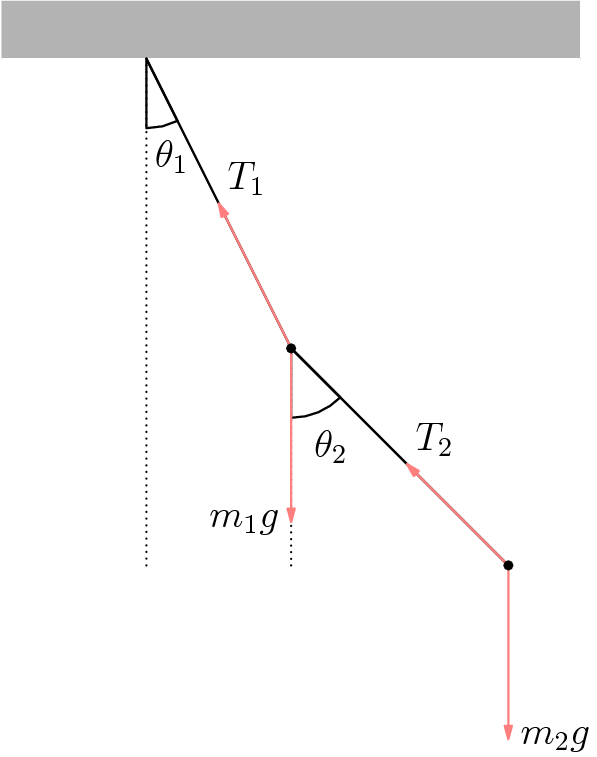
\includegraphics[width=8cm]{P03/double pendulum.png}
\end{center}
Since the angles are small, it holds that 
\[\sin\theta \approx \theta, \quad \cos\theta \approx 1.\]
Let us also define 
\[\sin\theta_1 = \frac{X_1}{L}, \quad \sin\theta_2 = \frac{X_2 - X_1}{L}.\]
The angles are small so $T_1 \approx (M_1 + M_2)g$ (as it holds both masses) and $T_2 \approx M_2 g$ (as it holds only the mass $M_2$). We can now write our equations of motion. We can start with the lower mass. The only force that attempts to bring the second mass back to
equilibrium is the horizontal component of $T_2$. Therefore, we have
\[M_2 \ddot{X}_2  = -T_2\sin\theta_2 = -\frac{M_2g}{\ell} (X_2 - X_1).\]
If we define $\omega^2 \equiv g/L$, we find 
\[\ddot{X}_2 + \omega_0^2 X_2 - \omega_0^2 X_1 = 0.\]
For the first mass, we have two forces. Although not labeled in the diagram there is a component $T_2$ that is directed along the rod and away from the first mass. Therefore, the two forces $T_1$ and $T_2$ fight for equilibrium and our equation of motion can be given as 
\begin{align*}
    M_1\ddot{X}_1 &= -T_1 \sin\theta_1 + T_2 \sin \theta_2 \\ 
     M_1 \ddot{X}_1 &= -2(M_1 + M_2)g \frac{X_1}{L} + M_2g\frac{X_2 - X_1}{L} \\
   0 &= \ddot{X}_1 + \frac{M_1 + 2M_2}{M_1}X_1\omega_0^2 - \frac{M_2}{M_1}X_2 \omega_0^2 
\end{align*}

   \item Using the definition of a normal mode 
\[
\begin{pmatrix}
X_1 \\
X_2 
\end{pmatrix}
= 
\Re \left[
\begin{pmatrix}
A_1 \\
A_2 
\end{pmatrix}
e^{i (\omega t + \phi)}
\right]
\]
we can rearrange to find that 
\begin{align*}
    0 &= \left(\frac{M_1 + 2M_2}{M_1}\omega_0^2 - \omega^2\right)A_1 - \frac{M_2}{M_1}\omega_0^2 A_2\\
    0 &= -\omega_0^2 A_1 + \left(\omega_0^2 - \omega^2\right)
\end{align*}
Now, rewrite in matrix format 
\[
\begin{pmatrix}
 \frac{M_1 + 2M_2}{M_1}\omega_0^2 - \omega^2 & -\frac{M_2}{M_1}\omega_0^2 \\ 
 -\omega_0^2 & \omega_0^2 - \omega^2
\end{pmatrix}
\begin{pmatrix}
A_1 \\
A_2
\end{pmatrix}
=0.
\]
To get a solution, we need to solve the equation where the determinant of the left matrix is zero.
\[
\begin{vmatrix}
\frac{M_1 + 2M_2}{M_1}\omega_0^2 - \omega^2 & -\frac{M_2}{M_1}\omega_0^2 \\ 
 -\omega_0^2 & \omega_0^2 - \omega^2
\end{vmatrix}
= 0.
\]
\[\left(\frac{M_1 + 2M_2}{M_1}\omega_0^2 - \omega^2\right)\left(\omega_0^2 - \omega^2\right) - \frac{M_2}{M_1}\omega_0^4 = 0\]
Rearranging yields the equation 
\[\omega^4 - \frac{2 (M_1 + M_2)}{M_1}\omega_0^2 \omega^2 + \frac{M_1 + M_2}{M_1}\omega_0^4 = 0.\]
Using substitution tells us that the roots of this equation are 
$$ \omega^2 = \frac{(M_2+M_1) \pm \sqrt {M_2^2 + M_1M_2}}{M1} \omega_0^2 \implies \omega^2 = (1+\alpha) \pm \sqrt {1+ \alpha^2}$$
Here we used $\alpha = \frac{M_2}{M_1}$
\end{enumerate}
\end{sol}
\begin{sol}
The main argument of the stationary phase principle is that if the phase changes too quickly, the integral will cancel out over the function. Thus, where the function peaks, $\frac{\partial \phi}{\partial k} = 0$, where $\phi$ is the phase.
\begin{enumerate}[label=\textbf{(\alph*)}]
\item $$\Psi(x) = \int_{-\infty}^{\infty}\mathrm{d}k\;\exp(-L^2(k - k_0)^2 + ikx)  = \int_{-\infty}^{\infty}\mathrm{d}k\;\exp(-L^2k^2 + 2L^2kk_0 - L^2k_0^2 + ikx)$$The phase part of the exponent is the imaginary term, so:
$$\frac{\partial}{\partial k}(ikx) = ix = 0 \implies x = 0$$This can be confirmed by actually evaluating the integral:
\begin{align*}
\Psi(x) &= \int_{-\infty}^{\infty}\mathrm{d}k\;\exp(-L^2k^2 + (2L^2k_0 + ix)k- L^2k_0^2) \\
&= \sqrt{\frac{\pi}{L^2}}\exp(L^2k_0^2)\exp((2L^2k_0 + ix)^2/4L^2) \\
&= \frac{\sqrt{\pi}}{L}\exp(L^2k_0^2)\exp(L^2k_0^2)\exp(ik_0x)\exp(-x^2/4L^2)
\end{align*}
Notice that the last exponential term decays to zero as $x$ moves away from zero, proving our conclusion that the wavefunction peaks at $x = 0$

\item $$\Psi(x) = \int_{-\infty}^{\infty}\mathrm{d}k\;\exp(-L^2(k - k_0)^2-ikx_0+ikx)$$
The wave-function peaks when
$$\frac{\partial}{\partial k}(-ikx_0+ikx) = -ix_0+ix \implies x = x_0$$
Let us try to verify this by evaluating the integral:
\begin{align*}
\Psi(x) &= \int_{-\infty}^{\infty}\mathrm{d}k\;\exp(-L^2k^2 + (2L^2k_0 - ix_0 + ix)k - L^2k_0^2) \\
&= \sqrt{\frac{\pi}{L^2}}\exp(L^2k_0^2)\exp\left(\frac{2L^2k_0 -ix_0+ix)^2}{4L^2}\right) \\
&= \frac{\sqrt{\pi}}{L}\exp(L^2k_0^2)\exp(L^2k_0^2)\exp(ik_0(x-x_0))\exp\left(\frac{-(x-x_0)^2}{4L^2}\right)
% &= \sqrt{\frac{\pi}{L^2}}\exp(4L^4k^2k_0^2/4L^2) \\
% &= \frac{\sqrt{\pi}}{L}\exp(L^2k^2k_0^2)
\end{align*}
Clearly, this wavefunction peaks at $x=x_0$. The extra phase shift introduced simply slides it over by that factor. 
\end{enumerate}
\end{sol}
\begin{sol}
\begin{enumerate}[label=\textbf{(\alph*)}]
\item On displacing by a distance $x$ from the equilibrium position, both springs will have a spring force directed towards the equilibrium position. This means that we have $$F_{\text{net}}= -(2Kx + Kx)\hat{x} = -3Kx\hat{x}.$$ 
Now, we write Newton's second law, and get rid of $\hat{x}$ as all the forces are in the $x$-direction to yield
\[m\ddot{x} = -3Kx\implies \omega = \boxed{\sqrt{\frac{3K}{M}}}.\]
\item At mean position, $v = A\omega $. Therefore 
\[A= \frac{v}{\omega} = \boxed{{v}\sqrt{\frac{M}{3K}}}.\]
\item We know $$x = A \sin (\omega t + \phi).$$ From initial conditions we know that $\omega = \sqrt{\frac{3K}{M}}$, $A={v}\sqrt{\frac{M}{3K}}$, and $\phi = 0$. Therefore 
$$ x = \boxed{v\sqrt {\frac {M}{3K}} \sin \left( \sqrt {\frac{3K}{M}} t \right)}.$$
\item From the lecture, we see that we can write the position of the center of mass as the complex function 
\[z (t) = \Re \left[Ae^{i (\omega t + \phi)}\right].\]
From initial conditions we know that $\omega = \sqrt{\frac{3K}{M}}$, $A=v\sqrt{\frac{M}{3K}}$, and $\phi = 0$ and therefore we have,
\[z(t) = \boxed{\Re \left[v\sqrt{\frac{M}{3K}}e^{i\sqrt{\frac{3K}{M}}t}\right]}.\]
\end{enumerate}
\end{sol}
\begin{sol}
\begin{enumerate}[label=\textbf{(\alph*)}]
\item Notice that 
\[\int_{-\infty}^{\infty}\dd x |\Psi (x)|^2 = \int_{-\infty}^{\infty}\dd x \Psi (x) \Psi^{*}(x) = \int_{-\infty}^{\infty} \dd x \left( \int_{-\infty}^{\infty} \dd p \Phi (p) e^{ixp}\right)\left(\int_{-\infty}^{\infty} \dd p' \Phi^{*} (p') e^{-ixp'}\right).  \]
This can be rewritten with the dirac delta function, as $\int e^{ix (p - p')} = \delta (p - p')$, so 
\[\int_{-\infty}^{\infty}\dd x\int_{-\infty}^{\infty}\dd p \Phi (p) \int_{-\infty}^{\infty}\dd p' \Phi^{*} (p') \delta (p - p') = \int_{-\infty}^{\infty} \dd p |\Phi (p)|^2.\]
\item Using the standard normalization integral and taking into account the spherical symmetry of the situation: $$\int_{0}^{\infty}\left(Ne^{-r/a_0}\right)^24\pi r^2\;\mathrm{d}r = \int_{0}^{\infty}N^2e^{-2r/a_0}\;4\pi r^2\;\mathrm{d}r = \pi N^2a_0^3 = 1$$ Thus, $$N = \sqrt{\frac{1}{\pi a_0^3}}$$
Using Parseval's theorem gives us a normalization condition for momentum wavefunctions similar to the one used in part b): $$\int_{-\infty}^{\infty}\frac{N'^2}{\left(1 + \frac{a_0^2p^2}{\hbar^2}\right)^4}\;4\pi p^2\;\mathrm{d}p = 1$$ Then, $$\int_{-\infty}^{\infty}\frac{4\pi p^2\;\mathrm{d}p}{\left(1 + \frac{a_0^2p^2}{\hbar^2}\right)^4} = \frac{\pi^2\hbar^3}{8a_0^3} \implies N' = \sqrt{\frac{8a_0^3}{\pi^2\hbar^3}}$$
Using the probabalistic interpretation of the momentum wavefunction, the probability that the \textbf{magnitude} of the momentum exceeds $\hbar/a_0$ is: $$\int_{\hbar/a_0}^{\infty}\frac{N'^2}{\left(1 + \frac{a_0^2p^2}{\hbar^2}\right)^4}\;4\pi p^2\;\mathrm{d}p$$
\end{enumerate}
\end{sol}
\begin{sol}
$|\gamma(t)|$ will continue increasing as the two wavepackets evolve, since their wavefunctions will have more overlap as they spread out.
\end{sol}
\begin{sol}
First note that: $$ J(x) = \frac{\hbar}{m}\operatorname{Im}(\Psi^*(x)\frac{\partial \Psi(x)}{\partial x}) = \frac{\hbar}{2im}(\Psi^*(x)\frac{\partial \Psi(x)}{\partial x} - \Psi(x)\frac{\partial \Psi^*(x)}{\partial x})$$
Then,
\begin{enumerate}[label=\textbf{(\alph*)}]
\item $\Psi(x) = Ae^{\gamma x}$:
\begin{align*}J(x) &= \frac{\hbar}{2im}(A^*e^{\gamma x}\frac{\partial }{\partial x}(Ae^{\gamma x}) - Ae^{\gamma x}\frac{\partial}{\partial x}(A^*e^{\gamma x})) \\ &= \frac{\hbar|A|^2}{2im}(e^{\gamma x}\frac{\partial}{\partial x}(e^{\gamma x}) - e^{\gamma x}\frac{\partial}{\partial x}(e^{\gamma x})) \\ &= 0
\end{align*}
Alternatively,
\begin{align*}
    J(x) &= \frac{\hbar}{m}\operatorname{Im}(A^*e^{\gamma x}\frac{\partial}{\partial x}(Ae^{\gamma x})) \\ &= \frac{\hbar}{m}\operatorname{Im}(AA^*\gamma e^{2\gamma x}) \\ &= 0
\end{align*}
\item $\Psi(x) = N(x)e^{iS(x)/\hbar}$:
\begin{align*}
    J(x) &= \frac{\hbar}{2im}(N(x)e^{-iS(x)/\hbar}\frac{\partial}{\partial x}(N(x)e^{iS(x)/\hbar}) - N(x)e^{iS(x)/\hbar}\frac{\partial}{\partial x}(N(x)e^{-iS(x)/\hbar})) \\ &= \frac{1}{m}N(x)^2\frac{\partial S(x)}{\partial x}
\end{align*}
Alternatively,
\begin{align*}
    J(x) &= \frac{\hbar}{m}\operatorname{Im}(N(x)e^{-iS(x)/\hbar}\frac{\partial}{\partial x}(N(x)e^{iS(x)/\hbar})) \\ &= \frac{\hbar}{m}\operatorname{Im}(N(x)^2 * i\frac{\partial S(x)}{\partial x}/\hbar) \\ &= \frac{1}{m}N(x)^2\frac{\partial S(x)}{\partial x}
\end{align*}
\item $\Psi(x) = Ae^{ikx} + Be^{-ikx}$:
\begin{align*}
    J(x) &= \frac{\hbar}{2im}((A^*e^{-ikx} + B^*e^{ikx})\frac{\partial}{\partial x}(Ae^{ikx} + Be^{-ikx}) - (Ae^{ikx} + Be^{-ikx})\frac{\partial}{\partial x}(A^*e^{-ikx} + B^*e^{ikx})) \\ &= \frac{\hbar k}{m}(AA^* - BB^*) \\ &= \frac{\hbar k}{m}(|A|^2 - |B|^2)
\end{align*}
Alternatively,
\begin{align*}
    J(x) &= \frac{\hbar}{m}\operatorname{Im}((A^*e^{-ikx} + B^*e^{ikx})\frac{\partial}{\partial x}(Ae^{ikx} + Be^{-ikx})) \\ &= \frac{\hbar}{m}(AA^* - BB^*) \\ &= \frac{\hbar}{m}(|A|^2 - |B|^2)
\end{align*}

\end{enumerate}
\end{sol}
\begin{sol}
\begin{enumerate}[label=\textbf{(\alph*)}]
\item First, note that:
\begin{align*}
    x_0 &= \left<x\right>_{\psi_0} = \int_{-\infty}^{\infty}\psi_0^*(x)\hat{x}\psi_0(x)\;\mathrm{d}x = \int_{-\infty}^{\infty}\psi_0^*(x)x\psi_0(x)\;\mathrm{d}x \\ p_0 &= \left<p\right>_{\psi_0} = \int_{-\infty}^{\infty}\psi_0^*(x)\hat{p}\psi_0(x)\;\mathrm{d}x = -i\hbar\int_{-\infty}^{\infty}\psi_0^*(x)\frac{\partial}{\partial x}\psi_0(x)\;\mathrm{d}x
\end{align*}
Now, in order to calculate the expectation values of the new wavefunction, first note that: $$\psi_{new}(x) = \hat{B_q}\psi(x) = e^{iqx/\hbar}\;\psi_0(x)$$\item
\begin{align*}
\left<x\right>_{\psi_{new}} &= \int_{-\infty}^{\infty}\psi_{new}^*(x)\hat{x}\psi_{new}(x) \;\mathrm{d}x \\ &= \int_{-\infty}^{\infty}\psi_0^*(x)e^{-iqx/\hbar}x\psi_0(x)e^{iqx/\hbar}\;\mathrm{d}x \\ &= \int_{-\infty}^{\infty}\psi_0^*(x)x\psi_0(x)\;\mathrm{d}x \\ &= x_0
\end{align*}
\item
\begin{align*}
\left<p\right>_{\psi_{new}} &= \int_{-\infty}^{\infty}\psi_{new}^*(x)\hat{p}\psi_{new}(x) \;\mathrm{d}x \\ &= \int_{-\infty}^{\infty}\psi_0^*(x)e^{-iqx/\hbar}\hat{p}\psi_0(x)e^{iqx/\hbar}\;\mathrm{d}x \\ &= \int_{-\infty}^{\infty}\psi_0^*(x)e^{-iqx/\hbar}(-i\hbar\frac{\partial}{\partial x})\psi_0(x)e^{iqx/\hbar}\;\mathrm{d}x \\ &= -i\hbar\int_{-\infty}^{\infty}\psi_0^*(x)e^{-iqx/\hbar}(e^{iqx/\hbar}\frac{\partial \psi_0(x)}{\partial x} + \frac{iq}{\hbar}e^{iqx/\hbar}\psi_0(x))\;\mathrm{d}x \\ &= -i\hbar\int_{-\infty}^{\infty}\psi_0^*(x)\frac{\partial}{\partial x}\psi_0(x)\;\mathrm{d}x + q\int_{-\infty}^{\infty}\psi_0^*(x)\psi_0(x)\;\mathrm{d}x \\ &= p_0 + q
\end{align*}
\item The boost operator has no effect on the measurement of the position, since the magnitude of the wavefunction is not changing (that is the only relevant matter when calculating a position-space probability distribution). However, the expected value of the momentum is "translated" by a constant value, based on the value $q$ of the boost operator.
\item For the momentum-boost commutator: $$[\hat{p}, \hat{B_q}]\psi(x) = \hat{p}\hat{B_q}\psi(x) - \hat{B_q}\hat{p}\psi(x) = -i\hbar\frac{\partial}{\partial x}\left(e^{iqx/\hbar}\psi(x)\right) - e^{iqx/\hbar}(-i\hbar)\frac{\partial\psi(x)}{\partial x}$$ Using the product rule and expanding and cancelling terms: $$[\hat{p}, \hat{B_q}]\psi(x) = q\psi(x) \implies [\hat{p}, \hat{B_q}] = q$$ For the position-boost commutator: $$[\hat{x}, \hat{B_q}] = \hat{x}\hat{B_q} - \hat{B_q}\hat{x} = xe^{iqx/\hbar} - e^{iqx/\hbar}x = 0$$
\end{enumerate}
\end{sol}

\newpage
\section*{Problem Set 2}
\begin{sol}
\begin{enumerate}[label=\textbf{(\alph*)}] 
\item We begin by first drawing a diagram:
\begin{center}
    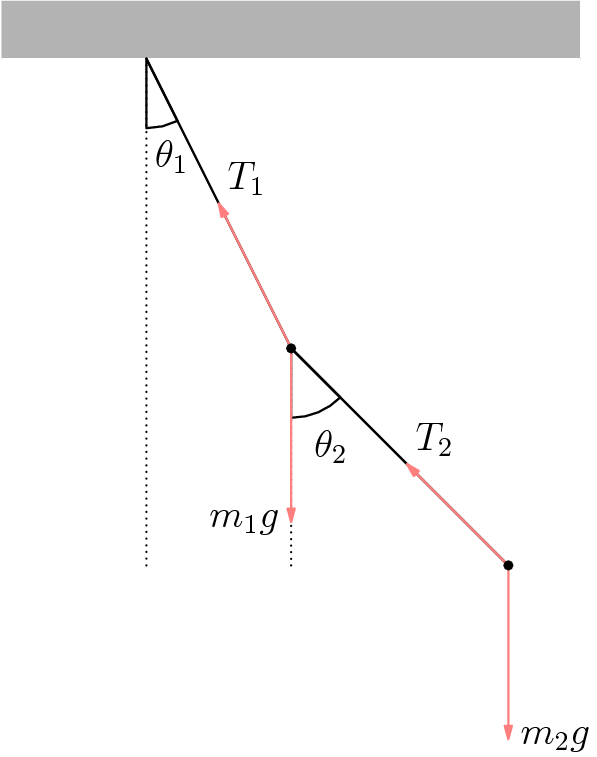
\includegraphics[width=8cm]{P03/double pendulum.png}
\end{center}
Since the angles are small, it holds that 
\[\sin\theta \approx \theta, \quad \cos\theta \approx 1.\]
Let us also define 
\[\sin\theta_1 = \frac{X_1}{L}, \quad \sin\theta_2 = \frac{X_2 - X_1}{L}.\]
The angles are small so $T_1 \approx (M_1 + M_2)g$ (as it holds both masses) and $T_2 \approx M_2 g$ (as it holds only the mass $M_2$). We can now write our equations of motion. We can start with the lower mass. The only force that attempts to bring the second mass back to
equilibrium is the horizontal component of $T_2$. Therefore, we have
\[M_2 \ddot{X}_2  = -T_2\sin\theta_2 = -\frac{M_2g}{\ell} (X_2 - X_1).\]
If we define $\omega^2 \equiv g/L$, we find 
\[\ddot{X}_2 + \omega_0^2 X_2 - \omega_0^2 X_1 = 0.\]
For the first mass, we have two forces. Although not labeled in the diagram there is a component $T_2$ that is directed along the rod and away from the first mass. Therefore, the two forces $T_1$ and $T_2$ fight for equilibrium and our equation of motion can be given as 
\begin{align*}
    M_1\ddot{X}_1 &= -T_1 \sin\theta_1 + T_2 \sin \theta_2 \\ 
     M_1 \ddot{X}_1 &= -2(M_1 + M_2)g \frac{X_1}{L} + M_2g\frac{X_2 - X_1}{L} \\
   0 &= \ddot{X}_1 + \frac{M_1 + 2M_2}{M_1}X_1\omega_0^2 - \frac{M_2}{M_1}X_2 \omega_0^2 
\end{align*}

   \item Using the definition of a normal mode 
\[
\begin{pmatrix}
X_1 \\
X_2 
\end{pmatrix}
= 
\Re \left[
\begin{pmatrix}
A_1 \\
A_2 
\end{pmatrix}
e^{i (\omega t + \phi)}
\right]
\]
we can rearrange to find that 
\begin{align*}
    0 &= \left(\frac{M_1 + 2M_2}{M_1}\omega_0^2 - \omega^2\right)A_1 - \frac{M_2}{M_1}\omega_0^2 A_2\\
    0 &= -\omega_0^2 A_1 + \left(\omega_0^2 - \omega^2\right)
\end{align*}
Now, rewrite in matrix format 
\[
\begin{pmatrix}
 \frac{M_1 + 2M_2}{M_1}\omega_0^2 - \omega^2 & -\frac{M_2}{M_1}\omega_0^2 \\ 
 -\omega_0^2 & \omega_0^2 - \omega^2
\end{pmatrix}
\begin{pmatrix}
A_1 \\
A_2
\end{pmatrix}
=0.
\]
To get a solution, we need to solve the equation where the determinant of the left matrix is zero.
\[
\begin{vmatrix}
\frac{M_1 + 2M_2}{M_1}\omega_0^2 - \omega^2 & -\frac{M_2}{M_1}\omega_0^2 \\ 
 -\omega_0^2 & \omega_0^2 - \omega^2
\end{vmatrix}
= 0.
\]
\[\left(\frac{M_1 + 2M_2}{M_1}\omega_0^2 - \omega^2\right)\left(\omega_0^2 - \omega^2\right) - \frac{M_2}{M_1}\omega_0^4 = 0\]
Rearranging yields the equation 
\[\omega^4 - \frac{2 (M_1 + M_2)}{M_1}\omega_0^2 \omega^2 + \frac{M_1 + M_2}{M_1}\omega_0^4 = 0.\]
Using substitution tells us that the roots of this equation are 
$$ \omega^2 = \frac{(M_2+M_1) \pm \sqrt {M_2^2 + M_1M_2}}{M1} \omega_0^2 \implies \omega^2 = (1+\alpha) \pm \sqrt {1+ \alpha^2}$$
Here we used $\alpha = \frac{M_2}{M_1}$
\end{enumerate}
\end{sol}
\begin{sol}
The main argument of the stationary phase principle is that if the phase changes too quickly, the integral will cancel out over the function. Thus, where the function peaks, $\frac{\partial \phi}{\partial k} = 0$, where $\phi$ is the phase.
\begin{enumerate}[label=\textbf{(\alph*)}]
\item $$\Psi(x) = \int_{-\infty}^{\infty}\mathrm{d}k\;\exp(-L^2(k - k_0)^2 + ikx)  = \int_{-\infty}^{\infty}\mathrm{d}k\;\exp(-L^2k^2 + 2L^2kk_0 - L^2k_0^2 + ikx)$$The phase part of the exponent is the imaginary term, so:
$$\frac{\partial}{\partial k}(ikx) = ix = 0 \implies x = 0$$This can be confirmed by actually evaluating the integral:
\begin{align*}
\Psi(x) &= \int_{-\infty}^{\infty}\mathrm{d}k\;\exp(-L^2k^2 + (2L^2k_0 + ix)k- L^2k_0^2) \\
&= \sqrt{\frac{\pi}{L^2}}\exp(L^2k_0^2)\exp((2L^2k_0 + ix)^2/4L^2) \\
&= \frac{\sqrt{\pi}}{L}\exp(L^2k_0^2)\exp(L^2k_0^2)\exp(ik_0x)\exp(-x^2/4L^2)
\end{align*}
Notice that the last exponential term decays to zero as $x$ moves away from zero, proving our conclusion that the wavefunction peaks at $x = 0$

\item $$\Psi(x) = \int_{-\infty}^{\infty}\mathrm{d}k\;\exp(-L^2(k - k_0)^2-ikx_0+ikx)$$
The wave-function peaks when
$$\frac{\partial}{\partial k}(-ikx_0+ikx) = -ix_0+ix \implies x = x_0$$
Let us try to verify this by evaluating the integral:
\begin{align*}
\Psi(x) &= \int_{-\infty}^{\infty}\mathrm{d}k\;\exp(-L^2k^2 + (2L^2k_0 - ix_0 + ix)k - L^2k_0^2) \\
&= \sqrt{\frac{\pi}{L^2}}\exp(L^2k_0^2)\exp\left(\frac{2L^2k_0 -ix_0+ix)^2}{4L^2}\right) \\
&= \frac{\sqrt{\pi}}{L}\exp(L^2k_0^2)\exp(L^2k_0^2)\exp(ik_0(x-x_0))\exp\left(\frac{-(x-x_0)^2}{4L^2}\right)
% &= \sqrt{\frac{\pi}{L^2}}\exp(4L^4k^2k_0^2/4L^2) \\
% &= \frac{\sqrt{\pi}}{L}\exp(L^2k^2k_0^2)
\end{align*}
Clearly, this wavefunction peaks at $x=x_0$. The extra phase shift introduced simply slides it over by that factor. 
\end{enumerate}
\end{sol}
\begin{sol}
\begin{enumerate}[label=\textbf{(\alph*)}]
\item On displacing by a distance $x$ from the equilibrium position, both springs will have a spring force directed towards the equilibrium position. This means that we have $$F_{\text{net}}= -(2Kx + Kx)\hat{x} = -3Kx\hat{x}.$$ 
Now, we write Newton's second law, and get rid of $\hat{x}$ as all the forces are in the $x$-direction to yield
\[m\ddot{x} = -3Kx\implies \omega = \boxed{\sqrt{\frac{3K}{M}}}.\]
\item At mean position, $v = A\omega $. Therefore 
\[A= \frac{v}{\omega} = \boxed{{v}\sqrt{\frac{M}{3K}}}.\]
\item We know $$x = A \sin (\omega t + \phi).$$ From initial conditions we know that $\omega = \sqrt{\frac{3K}{M}}$, $A={v}\sqrt{\frac{M}{3K}}$, and $\phi = 0$. Therefore 
$$ x = \boxed{v\sqrt {\frac {M}{3K}} \sin \left( \sqrt {\frac{3K}{M}} t \right)}.$$
\item From the lecture, we see that we can write the position of the center of mass as the complex function 
\[z (t) = \Re \left[Ae^{i (\omega t + \phi)}\right].\]
From initial conditions we know that $\omega = \sqrt{\frac{3K}{M}}$, $A=v\sqrt{\frac{M}{3K}}$, and $\phi = 0$ and therefore we have,
\[z(t) = \boxed{\Re \left[v\sqrt{\frac{M}{3K}}e^{i\sqrt{\frac{3K}{M}}t}\right]}.\]
\end{enumerate}
\end{sol}
\begin{sol}
\begin{enumerate}[label=\textbf{(\alph*)}]
\item Notice that 
\[\int_{-\infty}^{\infty}\dd x |\Psi (x)|^2 = \int_{-\infty}^{\infty}\dd x \Psi (x) \Psi^{*}(x) = \int_{-\infty}^{\infty} \dd x \left( \int_{-\infty}^{\infty} \dd p \Phi (p) e^{ixp}\right)\left(\int_{-\infty}^{\infty} \dd p' \Phi^{*} (p') e^{-ixp'}\right).  \]
This can be rewritten with the dirac delta function, as $\int e^{ix (p - p')} = \delta (p - p')$, so 
\[\int_{-\infty}^{\infty}\dd x\int_{-\infty}^{\infty}\dd p \Phi (p) \int_{-\infty}^{\infty}\dd p' \Phi^{*} (p') \delta (p - p') = \int_{-\infty}^{\infty} \dd p |\Phi (p)|^2.\]
\item Using the standard normalization integral and taking into account the spherical symmetry of the situation: $$\int_{0}^{\infty}\left(Ne^{-r/a_0}\right)^24\pi r^2\;\mathrm{d}r = \int_{0}^{\infty}N^2e^{-2r/a_0}\;4\pi r^2\;\mathrm{d}r = \pi N^2a_0^3 = 1$$ Thus, $$N = \sqrt{\frac{1}{\pi a_0^3}}$$
Using Parseval's theorem gives us a normalization condition for momentum wavefunctions similar to the one used in part b): $$\int_{-\infty}^{\infty}\frac{N'^2}{\left(1 + \frac{a_0^2p^2}{\hbar^2}\right)^4}\;4\pi p^2\;\mathrm{d}p = 1$$ Then, $$\int_{-\infty}^{\infty}\frac{4\pi p^2\;\mathrm{d}p}{\left(1 + \frac{a_0^2p^2}{\hbar^2}\right)^4} = \frac{\pi^2\hbar^3}{8a_0^3} \implies N' = \sqrt{\frac{8a_0^3}{\pi^2\hbar^3}}$$
Using the probabalistic interpretation of the momentum wavefunction, the probability that the \textbf{magnitude} of the momentum exceeds $\hbar/a_0$ is: $$\int_{\hbar/a_0}^{\infty}\frac{N'^2}{\left(1 + \frac{a_0^2p^2}{\hbar^2}\right)^4}\;4\pi p^2\;\mathrm{d}p$$
\end{enumerate}
\end{sol}
\begin{sol}
$|\gamma(t)|$ will continue increasing as the two wavepackets evolve, since their wavefunctions will have more overlap as they spread out.
\end{sol}

\newpage
\section*{Problem Set 3}
\begin{sol}
\begin{enumerate}[label=\textbf{(\alph*)}] 
\item We begin by first drawing a diagram:
\begin{center}
    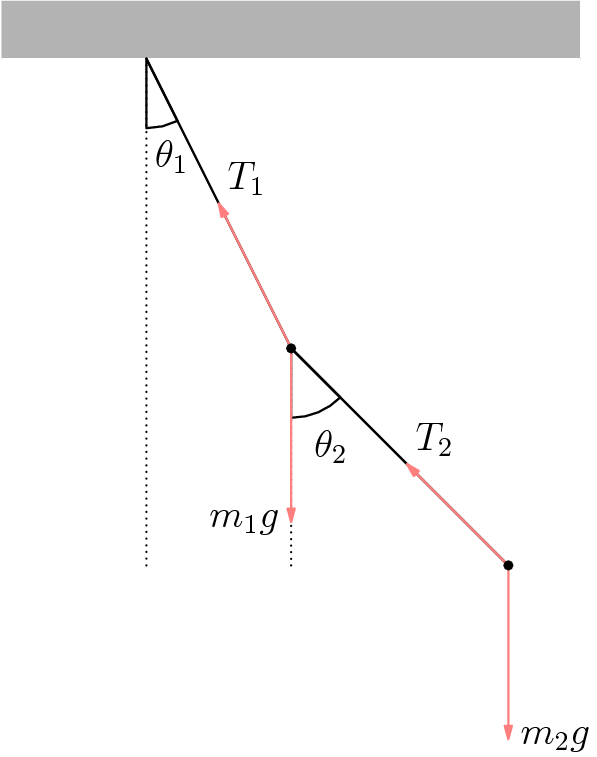
\includegraphics[width=8cm]{P03/double pendulum.png}
\end{center}
Since the angles are small, it holds that 
\[\sin\theta \approx \theta, \quad \cos\theta \approx 1.\]
Let us also define 
\[\sin\theta_1 = \frac{X_1}{L}, \quad \sin\theta_2 = \frac{X_2 - X_1}{L}.\]
The angles are small so $T_1 \approx (M_1 + M_2)g$ (as it holds both masses) and $T_2 \approx M_2 g$ (as it holds only the mass $M_2$). We can now write our equations of motion. We can start with the lower mass. The only force that attempts to bring the second mass back to
equilibrium is the horizontal component of $T_2$. Therefore, we have
\[M_2 \ddot{X}_2  = -T_2\sin\theta_2 = -\frac{M_2g}{\ell} (X_2 - X_1).\]
If we define $\omega^2 \equiv g/L$, we find 
\[\ddot{X}_2 + \omega_0^2 X_2 - \omega_0^2 X_1 = 0.\]
For the first mass, we have two forces. Although not labeled in the diagram there is a component $T_2$ that is directed along the rod and away from the first mass. Therefore, the two forces $T_1$ and $T_2$ fight for equilibrium and our equation of motion can be given as 
\begin{align*}
    M_1\ddot{X}_1 &= -T_1 \sin\theta_1 + T_2 \sin \theta_2 \\ 
     M_1 \ddot{X}_1 &= -2(M_1 + M_2)g \frac{X_1}{L} + M_2g\frac{X_2 - X_1}{L} \\
   0 &= \ddot{X}_1 + \frac{M_1 + 2M_2}{M_1}X_1\omega_0^2 - \frac{M_2}{M_1}X_2 \omega_0^2 
\end{align*}

   \item Using the definition of a normal mode 
\[
\begin{pmatrix}
X_1 \\
X_2 
\end{pmatrix}
= 
\Re \left[
\begin{pmatrix}
A_1 \\
A_2 
\end{pmatrix}
e^{i (\omega t + \phi)}
\right]
\]
we can rearrange to find that 
\begin{align*}
    0 &= \left(\frac{M_1 + 2M_2}{M_1}\omega_0^2 - \omega^2\right)A_1 - \frac{M_2}{M_1}\omega_0^2 A_2\\
    0 &= -\omega_0^2 A_1 + \left(\omega_0^2 - \omega^2\right)
\end{align*}
Now, rewrite in matrix format 
\[
\begin{pmatrix}
 \frac{M_1 + 2M_2}{M_1}\omega_0^2 - \omega^2 & -\frac{M_2}{M_1}\omega_0^2 \\ 
 -\omega_0^2 & \omega_0^2 - \omega^2
\end{pmatrix}
\begin{pmatrix}
A_1 \\
A_2
\end{pmatrix}
=0.
\]
To get a solution, we need to solve the equation where the determinant of the left matrix is zero.
\[
\begin{vmatrix}
\frac{M_1 + 2M_2}{M_1}\omega_0^2 - \omega^2 & -\frac{M_2}{M_1}\omega_0^2 \\ 
 -\omega_0^2 & \omega_0^2 - \omega^2
\end{vmatrix}
= 0.
\]
\[\left(\frac{M_1 + 2M_2}{M_1}\omega_0^2 - \omega^2\right)\left(\omega_0^2 - \omega^2\right) - \frac{M_2}{M_1}\omega_0^4 = 0\]
Rearranging yields the equation 
\[\omega^4 - \frac{2 (M_1 + M_2)}{M_1}\omega_0^2 \omega^2 + \frac{M_1 + M_2}{M_1}\omega_0^4 = 0.\]
Using substitution tells us that the roots of this equation are 
$$ \omega^2 = \frac{(M_2+M_1) \pm \sqrt {M_2^2 + M_1M_2}}{M1} \omega_0^2 \implies \omega^2 = (1+\alpha) \pm \sqrt {1+ \alpha^2}$$
Here we used $\alpha = \frac{M_2}{M_1}$
\end{enumerate}
\end{sol}
\begin{sol}
The main argument of the stationary phase principle is that if the phase changes too quickly, the integral will cancel out over the function. Thus, where the function peaks, $\frac{\partial \phi}{\partial k} = 0$, where $\phi$ is the phase.
\begin{enumerate}[label=\textbf{(\alph*)}]
\item $$\Psi(x) = \int_{-\infty}^{\infty}\mathrm{d}k\;\exp(-L^2(k - k_0)^2 + ikx)  = \int_{-\infty}^{\infty}\mathrm{d}k\;\exp(-L^2k^2 + 2L^2kk_0 - L^2k_0^2 + ikx)$$The phase part of the exponent is the imaginary term, so:
$$\frac{\partial}{\partial k}(ikx) = ix = 0 \implies x = 0$$This can be confirmed by actually evaluating the integral:
\begin{align*}
\Psi(x) &= \int_{-\infty}^{\infty}\mathrm{d}k\;\exp(-L^2k^2 + (2L^2k_0 + ix)k- L^2k_0^2) \\
&= \sqrt{\frac{\pi}{L^2}}\exp(L^2k_0^2)\exp((2L^2k_0 + ix)^2/4L^2) \\
&= \frac{\sqrt{\pi}}{L}\exp(L^2k_0^2)\exp(L^2k_0^2)\exp(ik_0x)\exp(-x^2/4L^2)
\end{align*}
Notice that the last exponential term decays to zero as $x$ moves away from zero, proving our conclusion that the wavefunction peaks at $x = 0$

\item $$\Psi(x) = \int_{-\infty}^{\infty}\mathrm{d}k\;\exp(-L^2(k - k_0)^2-ikx_0+ikx)$$
The wave-function peaks when
$$\frac{\partial}{\partial k}(-ikx_0+ikx) = -ix_0+ix \implies x = x_0$$
Let us try to verify this by evaluating the integral:
\begin{align*}
\Psi(x) &= \int_{-\infty}^{\infty}\mathrm{d}k\;\exp(-L^2k^2 + (2L^2k_0 - ix_0 + ix)k - L^2k_0^2) \\
&= \sqrt{\frac{\pi}{L^2}}\exp(L^2k_0^2)\exp\left(\frac{2L^2k_0 -ix_0+ix)^2}{4L^2}\right) \\
&= \frac{\sqrt{\pi}}{L}\exp(L^2k_0^2)\exp(L^2k_0^2)\exp(ik_0(x-x_0))\exp\left(\frac{-(x-x_0)^2}{4L^2}\right)
% &= \sqrt{\frac{\pi}{L^2}}\exp(4L^4k^2k_0^2/4L^2) \\
% &= \frac{\sqrt{\pi}}{L}\exp(L^2k^2k_0^2)
\end{align*}
Clearly, this wavefunction peaks at $x=x_0$. The extra phase shift introduced simply slides it over by that factor. 
\end{enumerate}
\end{sol}
\begin{sol}
\begin{enumerate}[label=\textbf{(\alph*)}]
\item On displacing by a distance $x$ from the equilibrium position, both springs will have a spring force directed towards the equilibrium position. This means that we have $$F_{\text{net}}= -(2Kx + Kx)\hat{x} = -3Kx\hat{x}.$$ 
Now, we write Newton's second law, and get rid of $\hat{x}$ as all the forces are in the $x$-direction to yield
\[m\ddot{x} = -3Kx\implies \omega = \boxed{\sqrt{\frac{3K}{M}}}.\]
\item At mean position, $v = A\omega $. Therefore 
\[A= \frac{v}{\omega} = \boxed{{v}\sqrt{\frac{M}{3K}}}.\]
\item We know $$x = A \sin (\omega t + \phi).$$ From initial conditions we know that $\omega = \sqrt{\frac{3K}{M}}$, $A={v}\sqrt{\frac{M}{3K}}$, and $\phi = 0$. Therefore 
$$ x = \boxed{v\sqrt {\frac {M}{3K}} \sin \left( \sqrt {\frac{3K}{M}} t \right)}.$$
\item From the lecture, we see that we can write the position of the center of mass as the complex function 
\[z (t) = \Re \left[Ae^{i (\omega t + \phi)}\right].\]
From initial conditions we know that $\omega = \sqrt{\frac{3K}{M}}$, $A=v\sqrt{\frac{M}{3K}}$, and $\phi = 0$ and therefore we have,
\[z(t) = \boxed{\Re \left[v\sqrt{\frac{M}{3K}}e^{i\sqrt{\frac{3K}{M}}t}\right]}.\]
\end{enumerate}
\end{sol}
\begin{sol}
\begin{enumerate}[label=\textbf{(\alph*)}]
\item Notice that 
\[\int_{-\infty}^{\infty}\dd x |\Psi (x)|^2 = \int_{-\infty}^{\infty}\dd x \Psi (x) \Psi^{*}(x) = \int_{-\infty}^{\infty} \dd x \left( \int_{-\infty}^{\infty} \dd p \Phi (p) e^{ixp}\right)\left(\int_{-\infty}^{\infty} \dd p' \Phi^{*} (p') e^{-ixp'}\right).  \]
This can be rewritten with the dirac delta function, as $\int e^{ix (p - p')} = \delta (p - p')$, so 
\[\int_{-\infty}^{\infty}\dd x\int_{-\infty}^{\infty}\dd p \Phi (p) \int_{-\infty}^{\infty}\dd p' \Phi^{*} (p') \delta (p - p') = \int_{-\infty}^{\infty} \dd p |\Phi (p)|^2.\]
\item Using the standard normalization integral and taking into account the spherical symmetry of the situation: $$\int_{0}^{\infty}\left(Ne^{-r/a_0}\right)^24\pi r^2\;\mathrm{d}r = \int_{0}^{\infty}N^2e^{-2r/a_0}\;4\pi r^2\;\mathrm{d}r = \pi N^2a_0^3 = 1$$ Thus, $$N = \sqrt{\frac{1}{\pi a_0^3}}$$
Using Parseval's theorem gives us a normalization condition for momentum wavefunctions similar to the one used in part b): $$\int_{-\infty}^{\infty}\frac{N'^2}{\left(1 + \frac{a_0^2p^2}{\hbar^2}\right)^4}\;4\pi p^2\;\mathrm{d}p = 1$$ Then, $$\int_{-\infty}^{\infty}\frac{4\pi p^2\;\mathrm{d}p}{\left(1 + \frac{a_0^2p^2}{\hbar^2}\right)^4} = \frac{\pi^2\hbar^3}{8a_0^3} \implies N' = \sqrt{\frac{8a_0^3}{\pi^2\hbar^3}}$$
Using the probabalistic interpretation of the momentum wavefunction, the probability that the \textbf{magnitude} of the momentum exceeds $\hbar/a_0$ is: $$\int_{\hbar/a_0}^{\infty}\frac{N'^2}{\left(1 + \frac{a_0^2p^2}{\hbar^2}\right)^4}\;4\pi p^2\;\mathrm{d}p$$
\end{enumerate}
\end{sol}
\begin{sol}
$|\gamma(t)|$ will continue increasing as the two wavepackets evolve, since their wavefunctions will have more overlap as they spread out.
\end{sol}
\begin{sol}
First note that: $$ J(x) = \frac{\hbar}{m}\operatorname{Im}(\Psi^*(x)\frac{\partial \Psi(x)}{\partial x}) = \frac{\hbar}{2im}(\Psi^*(x)\frac{\partial \Psi(x)}{\partial x} - \Psi(x)\frac{\partial \Psi^*(x)}{\partial x})$$
Then,
\begin{enumerate}[label=\textbf{(\alph*)}]
\item $\Psi(x) = Ae^{\gamma x}$:
\begin{align*}J(x) &= \frac{\hbar}{2im}(A^*e^{\gamma x}\frac{\partial }{\partial x}(Ae^{\gamma x}) - Ae^{\gamma x}\frac{\partial}{\partial x}(A^*e^{\gamma x})) \\ &= \frac{\hbar|A|^2}{2im}(e^{\gamma x}\frac{\partial}{\partial x}(e^{\gamma x}) - e^{\gamma x}\frac{\partial}{\partial x}(e^{\gamma x})) \\ &= 0
\end{align*}
Alternatively,
\begin{align*}
    J(x) &= \frac{\hbar}{m}\operatorname{Im}(A^*e^{\gamma x}\frac{\partial}{\partial x}(Ae^{\gamma x})) \\ &= \frac{\hbar}{m}\operatorname{Im}(AA^*\gamma e^{2\gamma x}) \\ &= 0
\end{align*}
\item $\Psi(x) = N(x)e^{iS(x)/\hbar}$:
\begin{align*}
    J(x) &= \frac{\hbar}{2im}(N(x)e^{-iS(x)/\hbar}\frac{\partial}{\partial x}(N(x)e^{iS(x)/\hbar}) - N(x)e^{iS(x)/\hbar}\frac{\partial}{\partial x}(N(x)e^{-iS(x)/\hbar})) \\ &= \frac{1}{m}N(x)^2\frac{\partial S(x)}{\partial x}
\end{align*}
Alternatively,
\begin{align*}
    J(x) &= \frac{\hbar}{m}\operatorname{Im}(N(x)e^{-iS(x)/\hbar}\frac{\partial}{\partial x}(N(x)e^{iS(x)/\hbar})) \\ &= \frac{\hbar}{m}\operatorname{Im}(N(x)^2 * i\frac{\partial S(x)}{\partial x}/\hbar) \\ &= \frac{1}{m}N(x)^2\frac{\partial S(x)}{\partial x}
\end{align*}
\item $\Psi(x) = Ae^{ikx} + Be^{-ikx}$:
\begin{align*}
    J(x) &= \frac{\hbar}{2im}((A^*e^{-ikx} + B^*e^{ikx})\frac{\partial}{\partial x}(Ae^{ikx} + Be^{-ikx}) - (Ae^{ikx} + Be^{-ikx})\frac{\partial}{\partial x}(A^*e^{-ikx} + B^*e^{ikx})) \\ &= \frac{\hbar k}{m}(AA^* - BB^*) \\ &= \frac{\hbar k}{m}(|A|^2 - |B|^2)
\end{align*}
Alternatively,
\begin{align*}
    J(x) &= \frac{\hbar}{m}\operatorname{Im}((A^*e^{-ikx} + B^*e^{ikx})\frac{\partial}{\partial x}(Ae^{ikx} + Be^{-ikx})) \\ &= \frac{\hbar}{m}(AA^* - BB^*) \\ &= \frac{\hbar}{m}(|A|^2 - |B|^2)
\end{align*}

\end{enumerate}
\end{sol}

\newpage
\section*{Problem Set 4}
\begin{sol}
\begin{enumerate}[label=\textbf{(\alph*)}] 
\item We begin by first drawing a diagram:
\begin{center}
    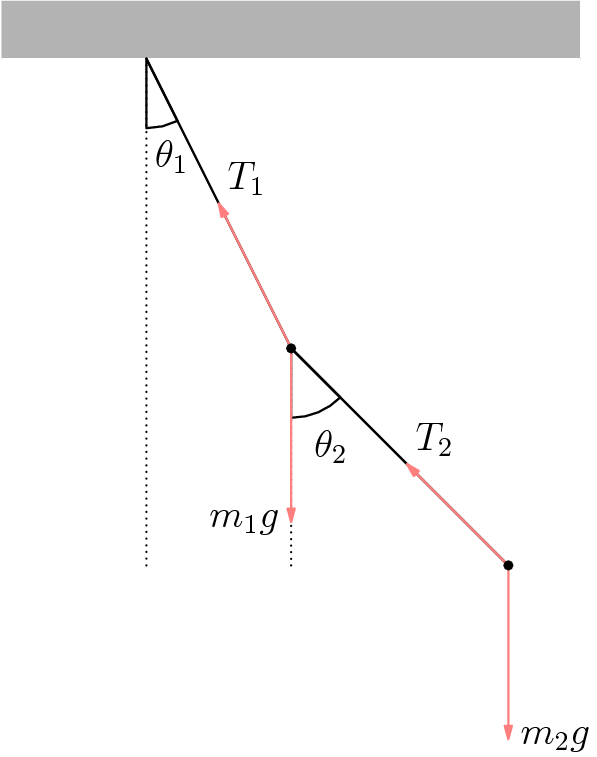
\includegraphics[width=8cm]{P03/double pendulum.png}
\end{center}
Since the angles are small, it holds that 
\[\sin\theta \approx \theta, \quad \cos\theta \approx 1.\]
Let us also define 
\[\sin\theta_1 = \frac{X_1}{L}, \quad \sin\theta_2 = \frac{X_2 - X_1}{L}.\]
The angles are small so $T_1 \approx (M_1 + M_2)g$ (as it holds both masses) and $T_2 \approx M_2 g$ (as it holds only the mass $M_2$). We can now write our equations of motion. We can start with the lower mass. The only force that attempts to bring the second mass back to
equilibrium is the horizontal component of $T_2$. Therefore, we have
\[M_2 \ddot{X}_2  = -T_2\sin\theta_2 = -\frac{M_2g}{\ell} (X_2 - X_1).\]
If we define $\omega^2 \equiv g/L$, we find 
\[\ddot{X}_2 + \omega_0^2 X_2 - \omega_0^2 X_1 = 0.\]
For the first mass, we have two forces. Although not labeled in the diagram there is a component $T_2$ that is directed along the rod and away from the first mass. Therefore, the two forces $T_1$ and $T_2$ fight for equilibrium and our equation of motion can be given as 
\begin{align*}
    M_1\ddot{X}_1 &= -T_1 \sin\theta_1 + T_2 \sin \theta_2 \\ 
     M_1 \ddot{X}_1 &= -2(M_1 + M_2)g \frac{X_1}{L} + M_2g\frac{X_2 - X_1}{L} \\
   0 &= \ddot{X}_1 + \frac{M_1 + 2M_2}{M_1}X_1\omega_0^2 - \frac{M_2}{M_1}X_2 \omega_0^2 
\end{align*}

   \item Using the definition of a normal mode 
\[
\begin{pmatrix}
X_1 \\
X_2 
\end{pmatrix}
= 
\Re \left[
\begin{pmatrix}
A_1 \\
A_2 
\end{pmatrix}
e^{i (\omega t + \phi)}
\right]
\]
we can rearrange to find that 
\begin{align*}
    0 &= \left(\frac{M_1 + 2M_2}{M_1}\omega_0^2 - \omega^2\right)A_1 - \frac{M_2}{M_1}\omega_0^2 A_2\\
    0 &= -\omega_0^2 A_1 + \left(\omega_0^2 - \omega^2\right)
\end{align*}
Now, rewrite in matrix format 
\[
\begin{pmatrix}
 \frac{M_1 + 2M_2}{M_1}\omega_0^2 - \omega^2 & -\frac{M_2}{M_1}\omega_0^2 \\ 
 -\omega_0^2 & \omega_0^2 - \omega^2
\end{pmatrix}
\begin{pmatrix}
A_1 \\
A_2
\end{pmatrix}
=0.
\]
To get a solution, we need to solve the equation where the determinant of the left matrix is zero.
\[
\begin{vmatrix}
\frac{M_1 + 2M_2}{M_1}\omega_0^2 - \omega^2 & -\frac{M_2}{M_1}\omega_0^2 \\ 
 -\omega_0^2 & \omega_0^2 - \omega^2
\end{vmatrix}
= 0.
\]
\[\left(\frac{M_1 + 2M_2}{M_1}\omega_0^2 - \omega^2\right)\left(\omega_0^2 - \omega^2\right) - \frac{M_2}{M_1}\omega_0^4 = 0\]
Rearranging yields the equation 
\[\omega^4 - \frac{2 (M_1 + M_2)}{M_1}\omega_0^2 \omega^2 + \frac{M_1 + M_2}{M_1}\omega_0^4 = 0.\]
Using substitution tells us that the roots of this equation are 
$$ \omega^2 = \frac{(M_2+M_1) \pm \sqrt {M_2^2 + M_1M_2}}{M1} \omega_0^2 \implies \omega^2 = (1+\alpha) \pm \sqrt {1+ \alpha^2}$$
Here we used $\alpha = \frac{M_2}{M_1}$
\end{enumerate}
\end{sol}
\begin{sol}
The main argument of the stationary phase principle is that if the phase changes too quickly, the integral will cancel out over the function. Thus, where the function peaks, $\frac{\partial \phi}{\partial k} = 0$, where $\phi$ is the phase.
\begin{enumerate}[label=\textbf{(\alph*)}]
\item $$\Psi(x) = \int_{-\infty}^{\infty}\mathrm{d}k\;\exp(-L^2(k - k_0)^2 + ikx)  = \int_{-\infty}^{\infty}\mathrm{d}k\;\exp(-L^2k^2 + 2L^2kk_0 - L^2k_0^2 + ikx)$$The phase part of the exponent is the imaginary term, so:
$$\frac{\partial}{\partial k}(ikx) = ix = 0 \implies x = 0$$This can be confirmed by actually evaluating the integral:
\begin{align*}
\Psi(x) &= \int_{-\infty}^{\infty}\mathrm{d}k\;\exp(-L^2k^2 + (2L^2k_0 + ix)k- L^2k_0^2) \\
&= \sqrt{\frac{\pi}{L^2}}\exp(L^2k_0^2)\exp((2L^2k_0 + ix)^2/4L^2) \\
&= \frac{\sqrt{\pi}}{L}\exp(L^2k_0^2)\exp(L^2k_0^2)\exp(ik_0x)\exp(-x^2/4L^2)
\end{align*}
Notice that the last exponential term decays to zero as $x$ moves away from zero, proving our conclusion that the wavefunction peaks at $x = 0$

\item $$\Psi(x) = \int_{-\infty}^{\infty}\mathrm{d}k\;\exp(-L^2(k - k_0)^2-ikx_0+ikx)$$
The wave-function peaks when
$$\frac{\partial}{\partial k}(-ikx_0+ikx) = -ix_0+ix \implies x = x_0$$
Let us try to verify this by evaluating the integral:
\begin{align*}
\Psi(x) &= \int_{-\infty}^{\infty}\mathrm{d}k\;\exp(-L^2k^2 + (2L^2k_0 - ix_0 + ix)k - L^2k_0^2) \\
&= \sqrt{\frac{\pi}{L^2}}\exp(L^2k_0^2)\exp\left(\frac{2L^2k_0 -ix_0+ix)^2}{4L^2}\right) \\
&= \frac{\sqrt{\pi}}{L}\exp(L^2k_0^2)\exp(L^2k_0^2)\exp(ik_0(x-x_0))\exp\left(\frac{-(x-x_0)^2}{4L^2}\right)
% &= \sqrt{\frac{\pi}{L^2}}\exp(4L^4k^2k_0^2/4L^2) \\
% &= \frac{\sqrt{\pi}}{L}\exp(L^2k^2k_0^2)
\end{align*}
Clearly, this wavefunction peaks at $x=x_0$. The extra phase shift introduced simply slides it over by that factor. 
\end{enumerate}
\end{sol}
\begin{sol}
\begin{enumerate}[label=\textbf{(\alph*)}]
\item On displacing by a distance $x$ from the equilibrium position, both springs will have a spring force directed towards the equilibrium position. This means that we have $$F_{\text{net}}= -(2Kx + Kx)\hat{x} = -3Kx\hat{x}.$$ 
Now, we write Newton's second law, and get rid of $\hat{x}$ as all the forces are in the $x$-direction to yield
\[m\ddot{x} = -3Kx\implies \omega = \boxed{\sqrt{\frac{3K}{M}}}.\]
\item At mean position, $v = A\omega $. Therefore 
\[A= \frac{v}{\omega} = \boxed{{v}\sqrt{\frac{M}{3K}}}.\]
\item We know $$x = A \sin (\omega t + \phi).$$ From initial conditions we know that $\omega = \sqrt{\frac{3K}{M}}$, $A={v}\sqrt{\frac{M}{3K}}$, and $\phi = 0$. Therefore 
$$ x = \boxed{v\sqrt {\frac {M}{3K}} \sin \left( \sqrt {\frac{3K}{M}} t \right)}.$$
\item From the lecture, we see that we can write the position of the center of mass as the complex function 
\[z (t) = \Re \left[Ae^{i (\omega t + \phi)}\right].\]
From initial conditions we know that $\omega = \sqrt{\frac{3K}{M}}$, $A=v\sqrt{\frac{M}{3K}}$, and $\phi = 0$ and therefore we have,
\[z(t) = \boxed{\Re \left[v\sqrt{\frac{M}{3K}}e^{i\sqrt{\frac{3K}{M}}t}\right]}.\]
\end{enumerate}
\end{sol}
\begin{sol}
\begin{enumerate}[label=\textbf{(\alph*)}]
\item Notice that 
\[\int_{-\infty}^{\infty}\dd x |\Psi (x)|^2 = \int_{-\infty}^{\infty}\dd x \Psi (x) \Psi^{*}(x) = \int_{-\infty}^{\infty} \dd x \left( \int_{-\infty}^{\infty} \dd p \Phi (p) e^{ixp}\right)\left(\int_{-\infty}^{\infty} \dd p' \Phi^{*} (p') e^{-ixp'}\right).  \]
This can be rewritten with the dirac delta function, as $\int e^{ix (p - p')} = \delta (p - p')$, so 
\[\int_{-\infty}^{\infty}\dd x\int_{-\infty}^{\infty}\dd p \Phi (p) \int_{-\infty}^{\infty}\dd p' \Phi^{*} (p') \delta (p - p') = \int_{-\infty}^{\infty} \dd p |\Phi (p)|^2.\]
\item Using the standard normalization integral and taking into account the spherical symmetry of the situation: $$\int_{0}^{\infty}\left(Ne^{-r/a_0}\right)^24\pi r^2\;\mathrm{d}r = \int_{0}^{\infty}N^2e^{-2r/a_0}\;4\pi r^2\;\mathrm{d}r = \pi N^2a_0^3 = 1$$ Thus, $$N = \sqrt{\frac{1}{\pi a_0^3}}$$
Using Parseval's theorem gives us a normalization condition for momentum wavefunctions similar to the one used in part b): $$\int_{-\infty}^{\infty}\frac{N'^2}{\left(1 + \frac{a_0^2p^2}{\hbar^2}\right)^4}\;4\pi p^2\;\mathrm{d}p = 1$$ Then, $$\int_{-\infty}^{\infty}\frac{4\pi p^2\;\mathrm{d}p}{\left(1 + \frac{a_0^2p^2}{\hbar^2}\right)^4} = \frac{\pi^2\hbar^3}{8a_0^3} \implies N' = \sqrt{\frac{8a_0^3}{\pi^2\hbar^3}}$$
Using the probabalistic interpretation of the momentum wavefunction, the probability that the \textbf{magnitude} of the momentum exceeds $\hbar/a_0$ is: $$\int_{\hbar/a_0}^{\infty}\frac{N'^2}{\left(1 + \frac{a_0^2p^2}{\hbar^2}\right)^4}\;4\pi p^2\;\mathrm{d}p$$
\end{enumerate}
\end{sol}
\begin{sol}
$|\gamma(t)|$ will continue increasing as the two wavepackets evolve, since their wavefunctions will have more overlap as they spread out.
\end{sol}
\newpage
\begin{sol}
First note that: $$ J(x) = \frac{\hbar}{m}\operatorname{Im}(\Psi^*(x)\frac{\partial \Psi(x)}{\partial x}) = \frac{\hbar}{2im}(\Psi^*(x)\frac{\partial \Psi(x)}{\partial x} - \Psi(x)\frac{\partial \Psi^*(x)}{\partial x})$$
Then,
\begin{enumerate}[label=\textbf{(\alph*)}]
\item $\Psi(x) = Ae^{\gamma x}$:
\begin{align*}J(x) &= \frac{\hbar}{2im}(A^*e^{\gamma x}\frac{\partial }{\partial x}(Ae^{\gamma x}) - Ae^{\gamma x}\frac{\partial}{\partial x}(A^*e^{\gamma x})) \\ &= \frac{\hbar|A|^2}{2im}(e^{\gamma x}\frac{\partial}{\partial x}(e^{\gamma x}) - e^{\gamma x}\frac{\partial}{\partial x}(e^{\gamma x})) \\ &= 0
\end{align*}
Alternatively,
\begin{align*}
    J(x) &= \frac{\hbar}{m}\operatorname{Im}(A^*e^{\gamma x}\frac{\partial}{\partial x}(Ae^{\gamma x})) \\ &= \frac{\hbar}{m}\operatorname{Im}(AA^*\gamma e^{2\gamma x}) \\ &= 0
\end{align*}
\item $\Psi(x) = N(x)e^{iS(x)/\hbar}$:
\begin{align*}
    J(x) &= \frac{\hbar}{2im}(N(x)e^{-iS(x)/\hbar}\frac{\partial}{\partial x}(N(x)e^{iS(x)/\hbar}) - N(x)e^{iS(x)/\hbar}\frac{\partial}{\partial x}(N(x)e^{-iS(x)/\hbar})) \\ &= \frac{1}{m}N(x)^2\frac{\partial S(x)}{\partial x}
\end{align*}
Alternatively,
\begin{align*}
    J(x) &= \frac{\hbar}{m}\operatorname{Im}(N(x)e^{-iS(x)/\hbar}\frac{\partial}{\partial x}(N(x)e^{iS(x)/\hbar})) \\ &= \frac{\hbar}{m}\operatorname{Im}(N(x)^2 * i\frac{\partial S(x)}{\partial x}/\hbar) \\ &= \frac{1}{m}N(x)^2\frac{\partial S(x)}{\partial x}
\end{align*}
\item $\Psi(x) = Ae^{ikx} + Be^{-ikx}$:
\begin{align*}
    J(x) &= \frac{\hbar}{2im}((A^*e^{-ikx} + B^*e^{ikx})\frac{\partial}{\partial x}(Ae^{ikx} + Be^{-ikx}) - (Ae^{ikx} + Be^{-ikx})\frac{\partial}{\partial x}(A^*e^{-ikx} + B^*e^{ikx})) \\ &= \frac{\hbar k}{m}(AA^* - BB^*) \\ &= \frac{\hbar k}{m}(|A|^2 - |B|^2)
\end{align*}
Alternatively,
\begin{align*}
    J(x) &= \frac{\hbar}{m}\operatorname{Im}((A^*e^{-ikx} + B^*e^{ikx})\frac{\partial}{\partial x}(Ae^{ikx} + Be^{-ikx})) \\ &= \frac{\hbar}{m}(AA^* - BB^*) \\ &= \frac{\hbar}{m}(|A|^2 - |B|^2)
\end{align*}

\end{enumerate}
\end{sol}
\begin{sol}
\begin{enumerate}[label=\textbf{(\alph*)}]
\item First, note that:
\begin{align*}
    x_0 &= \left<x\right>_{\psi_0} = \int_{-\infty}^{\infty}\psi_0^*(x)\hat{x}\psi_0(x)\;\mathrm{d}x = \int_{-\infty}^{\infty}\psi_0^*(x)x\psi_0(x)\;\mathrm{d}x \\ p_0 &= \left<p\right>_{\psi_0} = \int_{-\infty}^{\infty}\psi_0^*(x)\hat{p}\psi_0(x)\;\mathrm{d}x = -i\hbar\int_{-\infty}^{\infty}\psi_0^*(x)\frac{\partial}{\partial x}\psi_0(x)\;\mathrm{d}x
\end{align*}
Now, in order to calculate the expectation values of the new wavefunction, first note that: $$\psi_{new}(x) = \hat{B_q}\psi(x) = e^{iqx/\hbar}\;\psi_0(x)$$\item
\begin{align*}
\left<x\right>_{\psi_{new}} &= \int_{-\infty}^{\infty}\psi_{new}^*(x)\hat{x}\psi_{new}(x) \;\mathrm{d}x \\ &= \int_{-\infty}^{\infty}\psi_0^*(x)e^{-iqx/\hbar}x\psi_0(x)e^{iqx/\hbar}\;\mathrm{d}x \\ &= \int_{-\infty}^{\infty}\psi_0^*(x)x\psi_0(x)\;\mathrm{d}x \\ &= x_0
\end{align*}
\item
\begin{align*}
\left<p\right>_{\psi_{new}} &= \int_{-\infty}^{\infty}\psi_{new}^*(x)\hat{p}\psi_{new}(x) \;\mathrm{d}x \\ &= \int_{-\infty}^{\infty}\psi_0^*(x)e^{-iqx/\hbar}\hat{p}\psi_0(x)e^{iqx/\hbar}\;\mathrm{d}x \\ &= \int_{-\infty}^{\infty}\psi_0^*(x)e^{-iqx/\hbar}(-i\hbar\frac{\partial}{\partial x})\psi_0(x)e^{iqx/\hbar}\;\mathrm{d}x \\ &= -i\hbar\int_{-\infty}^{\infty}\psi_0^*(x)e^{-iqx/\hbar}(e^{iqx/\hbar}\frac{\partial \psi_0(x)}{\partial x} + \frac{iq}{\hbar}e^{iqx/\hbar}\psi_0(x))\;\mathrm{d}x \\ &= -i\hbar\int_{-\infty}^{\infty}\psi_0^*(x)\frac{\partial}{\partial x}\psi_0(x)\;\mathrm{d}x + q\int_{-\infty}^{\infty}\psi_0^*(x)\psi_0(x)\;\mathrm{d}x \\ &= p_0 + q
\end{align*}
\item The boost operator has no effect on the measurement of the position, since the magnitude of the wavefunction is not changing (that is the only relevant matter when calculating a position-space probability distribution). However, the expected value of the momentum is "translated" by a constant value, based on the value $q$ of the boost operator.
\item For the momentum-boost commutator: $$[\hat{p}, \hat{B_q}]\psi(x) = \hat{p}\hat{B_q}\psi(x) - \hat{B_q}\hat{p}\psi(x) = -i\hbar\frac{\partial}{\partial x}\left(e^{iqx/\hbar}\psi(x)\right) - e^{iqx/\hbar}(-i\hbar)\frac{\partial\psi(x)}{\partial x}$$ Using the product rule and expanding and cancelling terms: $$[\hat{p}, \hat{B_q}]\psi(x) = q\psi(x) \implies [\hat{p}, \hat{B_q}] = q$$ For the position-boost commutator: $$[\hat{x}, \hat{B_q}] = \hat{x}\hat{B_q} - \hat{B_q}\hat{x} = xe^{iqx/\hbar} - e^{iqx/\hbar}x = 0$$
\end{enumerate}
\end{sol}

\newpage
\section*{Problem Set 5}
\begin{sol}
\begin{enumerate}[label=\textbf{(\alph*)}] 
\item We begin by first drawing a diagram:
\begin{center}
    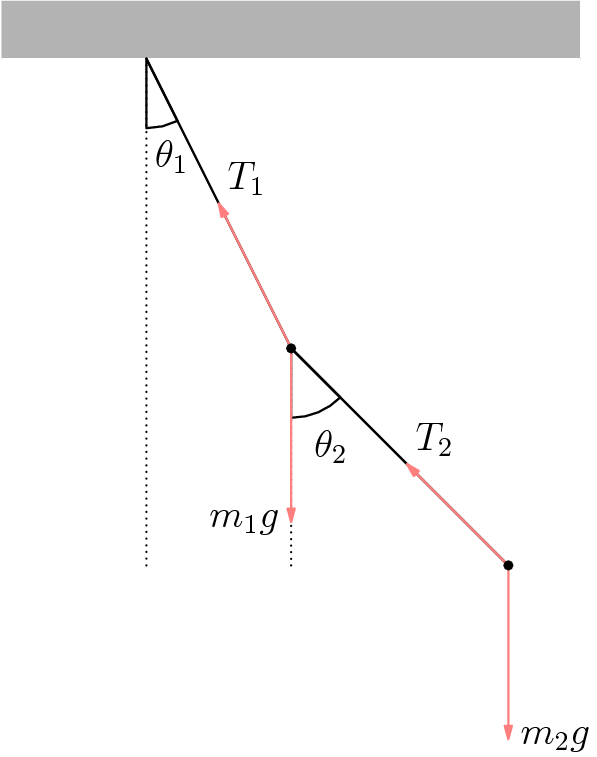
\includegraphics[width=8cm]{P03/double pendulum.png}
\end{center}
Since the angles are small, it holds that 
\[\sin\theta \approx \theta, \quad \cos\theta \approx 1.\]
Let us also define 
\[\sin\theta_1 = \frac{X_1}{L}, \quad \sin\theta_2 = \frac{X_2 - X_1}{L}.\]
The angles are small so $T_1 \approx (M_1 + M_2)g$ (as it holds both masses) and $T_2 \approx M_2 g$ (as it holds only the mass $M_2$). We can now write our equations of motion. We can start with the lower mass. The only force that attempts to bring the second mass back to
equilibrium is the horizontal component of $T_2$. Therefore, we have
\[M_2 \ddot{X}_2  = -T_2\sin\theta_2 = -\frac{M_2g}{\ell} (X_2 - X_1).\]
If we define $\omega^2 \equiv g/L$, we find 
\[\ddot{X}_2 + \omega_0^2 X_2 - \omega_0^2 X_1 = 0.\]
For the first mass, we have two forces. Although not labeled in the diagram there is a component $T_2$ that is directed along the rod and away from the first mass. Therefore, the two forces $T_1$ and $T_2$ fight for equilibrium and our equation of motion can be given as 
\begin{align*}
    M_1\ddot{X}_1 &= -T_1 \sin\theta_1 + T_2 \sin \theta_2 \\ 
     M_1 \ddot{X}_1 &= -2(M_1 + M_2)g \frac{X_1}{L} + M_2g\frac{X_2 - X_1}{L} \\
   0 &= \ddot{X}_1 + \frac{M_1 + 2M_2}{M_1}X_1\omega_0^2 - \frac{M_2}{M_1}X_2 \omega_0^2 
\end{align*}

   \item Using the definition of a normal mode 
\[
\begin{pmatrix}
X_1 \\
X_2 
\end{pmatrix}
= 
\Re \left[
\begin{pmatrix}
A_1 \\
A_2 
\end{pmatrix}
e^{i (\omega t + \phi)}
\right]
\]
we can rearrange to find that 
\begin{align*}
    0 &= \left(\frac{M_1 + 2M_2}{M_1}\omega_0^2 - \omega^2\right)A_1 - \frac{M_2}{M_1}\omega_0^2 A_2\\
    0 &= -\omega_0^2 A_1 + \left(\omega_0^2 - \omega^2\right)
\end{align*}
Now, rewrite in matrix format 
\[
\begin{pmatrix}
 \frac{M_1 + 2M_2}{M_1}\omega_0^2 - \omega^2 & -\frac{M_2}{M_1}\omega_0^2 \\ 
 -\omega_0^2 & \omega_0^2 - \omega^2
\end{pmatrix}
\begin{pmatrix}
A_1 \\
A_2
\end{pmatrix}
=0.
\]
To get a solution, we need to solve the equation where the determinant of the left matrix is zero.
\[
\begin{vmatrix}
\frac{M_1 + 2M_2}{M_1}\omega_0^2 - \omega^2 & -\frac{M_2}{M_1}\omega_0^2 \\ 
 -\omega_0^2 & \omega_0^2 - \omega^2
\end{vmatrix}
= 0.
\]
\[\left(\frac{M_1 + 2M_2}{M_1}\omega_0^2 - \omega^2\right)\left(\omega_0^2 - \omega^2\right) - \frac{M_2}{M_1}\omega_0^4 = 0\]
Rearranging yields the equation 
\[\omega^4 - \frac{2 (M_1 + M_2)}{M_1}\omega_0^2 \omega^2 + \frac{M_1 + M_2}{M_1}\omega_0^4 = 0.\]
Using substitution tells us that the roots of this equation are 
$$ \omega^2 = \frac{(M_2+M_1) \pm \sqrt {M_2^2 + M_1M_2}}{M1} \omega_0^2 \implies \omega^2 = (1+\alpha) \pm \sqrt {1+ \alpha^2}$$
Here we used $\alpha = \frac{M_2}{M_1}$
\end{enumerate}
\end{sol}
\begin{sol}
The main argument of the stationary phase principle is that if the phase changes too quickly, the integral will cancel out over the function. Thus, where the function peaks, $\frac{\partial \phi}{\partial k} = 0$, where $\phi$ is the phase.
\begin{enumerate}[label=\textbf{(\alph*)}]
\item $$\Psi(x) = \int_{-\infty}^{\infty}\mathrm{d}k\;\exp(-L^2(k - k_0)^2 + ikx)  = \int_{-\infty}^{\infty}\mathrm{d}k\;\exp(-L^2k^2 + 2L^2kk_0 - L^2k_0^2 + ikx)$$The phase part of the exponent is the imaginary term, so:
$$\frac{\partial}{\partial k}(ikx) = ix = 0 \implies x = 0$$This can be confirmed by actually evaluating the integral:
\begin{align*}
\Psi(x) &= \int_{-\infty}^{\infty}\mathrm{d}k\;\exp(-L^2k^2 + (2L^2k_0 + ix)k- L^2k_0^2) \\
&= \sqrt{\frac{\pi}{L^2}}\exp(L^2k_0^2)\exp((2L^2k_0 + ix)^2/4L^2) \\
&= \frac{\sqrt{\pi}}{L}\exp(L^2k_0^2)\exp(L^2k_0^2)\exp(ik_0x)\exp(-x^2/4L^2)
\end{align*}
Notice that the last exponential term decays to zero as $x$ moves away from zero, proving our conclusion that the wavefunction peaks at $x = 0$

\item $$\Psi(x) = \int_{-\infty}^{\infty}\mathrm{d}k\;\exp(-L^2(k - k_0)^2-ikx_0+ikx)$$
The wave-function peaks when
$$\frac{\partial}{\partial k}(-ikx_0+ikx) = -ix_0+ix \implies x = x_0$$
Let us try to verify this by evaluating the integral:
\begin{align*}
\Psi(x) &= \int_{-\infty}^{\infty}\mathrm{d}k\;\exp(-L^2k^2 + (2L^2k_0 - ix_0 + ix)k - L^2k_0^2) \\
&= \sqrt{\frac{\pi}{L^2}}\exp(L^2k_0^2)\exp\left(\frac{2L^2k_0 -ix_0+ix)^2}{4L^2}\right) \\
&= \frac{\sqrt{\pi}}{L}\exp(L^2k_0^2)\exp(L^2k_0^2)\exp(ik_0(x-x_0))\exp\left(\frac{-(x-x_0)^2}{4L^2}\right)
% &= \sqrt{\frac{\pi}{L^2}}\exp(4L^4k^2k_0^2/4L^2) \\
% &= \frac{\sqrt{\pi}}{L}\exp(L^2k^2k_0^2)
\end{align*}
Clearly, this wavefunction peaks at $x=x_0$. The extra phase shift introduced simply slides it over by that factor. 
\end{enumerate}
\end{sol}
\begin{sol}
\begin{enumerate}[label=\textbf{(\alph*)}]
\item On displacing by a distance $x$ from the equilibrium position, both springs will have a spring force directed towards the equilibrium position. This means that we have $$F_{\text{net}}= -(2Kx + Kx)\hat{x} = -3Kx\hat{x}.$$ 
Now, we write Newton's second law, and get rid of $\hat{x}$ as all the forces are in the $x$-direction to yield
\[m\ddot{x} = -3Kx\implies \omega = \boxed{\sqrt{\frac{3K}{M}}}.\]
\item At mean position, $v = A\omega $. Therefore 
\[A= \frac{v}{\omega} = \boxed{{v}\sqrt{\frac{M}{3K}}}.\]
\item We know $$x = A \sin (\omega t + \phi).$$ From initial conditions we know that $\omega = \sqrt{\frac{3K}{M}}$, $A={v}\sqrt{\frac{M}{3K}}$, and $\phi = 0$. Therefore 
$$ x = \boxed{v\sqrt {\frac {M}{3K}} \sin \left( \sqrt {\frac{3K}{M}} t \right)}.$$
\item From the lecture, we see that we can write the position of the center of mass as the complex function 
\[z (t) = \Re \left[Ae^{i (\omega t + \phi)}\right].\]
From initial conditions we know that $\omega = \sqrt{\frac{3K}{M}}$, $A=v\sqrt{\frac{M}{3K}}$, and $\phi = 0$ and therefore we have,
\[z(t) = \boxed{\Re \left[v\sqrt{\frac{M}{3K}}e^{i\sqrt{\frac{3K}{M}}t}\right]}.\]
\end{enumerate}
\end{sol}
\begin{sol}
\begin{enumerate}[label=\textbf{(\alph*)}]
\item Notice that 
\[\int_{-\infty}^{\infty}\dd x |\Psi (x)|^2 = \int_{-\infty}^{\infty}\dd x \Psi (x) \Psi^{*}(x) = \int_{-\infty}^{\infty} \dd x \left( \int_{-\infty}^{\infty} \dd p \Phi (p) e^{ixp}\right)\left(\int_{-\infty}^{\infty} \dd p' \Phi^{*} (p') e^{-ixp'}\right).  \]
This can be rewritten with the dirac delta function, as $\int e^{ix (p - p')} = \delta (p - p')$, so 
\[\int_{-\infty}^{\infty}\dd x\int_{-\infty}^{\infty}\dd p \Phi (p) \int_{-\infty}^{\infty}\dd p' \Phi^{*} (p') \delta (p - p') = \int_{-\infty}^{\infty} \dd p |\Phi (p)|^2.\]
\item Using the standard normalization integral and taking into account the spherical symmetry of the situation: $$\int_{0}^{\infty}\left(Ne^{-r/a_0}\right)^24\pi r^2\;\mathrm{d}r = \int_{0}^{\infty}N^2e^{-2r/a_0}\;4\pi r^2\;\mathrm{d}r = \pi N^2a_0^3 = 1$$ Thus, $$N = \sqrt{\frac{1}{\pi a_0^3}}$$
Using Parseval's theorem gives us a normalization condition for momentum wavefunctions similar to the one used in part b): $$\int_{-\infty}^{\infty}\frac{N'^2}{\left(1 + \frac{a_0^2p^2}{\hbar^2}\right)^4}\;4\pi p^2\;\mathrm{d}p = 1$$ Then, $$\int_{-\infty}^{\infty}\frac{4\pi p^2\;\mathrm{d}p}{\left(1 + \frac{a_0^2p^2}{\hbar^2}\right)^4} = \frac{\pi^2\hbar^3}{8a_0^3} \implies N' = \sqrt{\frac{8a_0^3}{\pi^2\hbar^3}}$$
Using the probabalistic interpretation of the momentum wavefunction, the probability that the \textbf{magnitude} of the momentum exceeds $\hbar/a_0$ is: $$\int_{\hbar/a_0}^{\infty}\frac{N'^2}{\left(1 + \frac{a_0^2p^2}{\hbar^2}\right)^4}\;4\pi p^2\;\mathrm{d}p$$
\end{enumerate}
\end{sol}
\begin{sol}
$|\gamma(t)|$ will continue increasing as the two wavepackets evolve, since their wavefunctions will have more overlap as they spread out.
\end{sol}
\begin{sol}
First note that: $$ J(x) = \frac{\hbar}{m}\operatorname{Im}(\Psi^*(x)\frac{\partial \Psi(x)}{\partial x}) = \frac{\hbar}{2im}(\Psi^*(x)\frac{\partial \Psi(x)}{\partial x} - \Psi(x)\frac{\partial \Psi^*(x)}{\partial x})$$
Then,
\begin{enumerate}[label=\textbf{(\alph*)}]
\item $\Psi(x) = Ae^{\gamma x}$:
\begin{align*}J(x) &= \frac{\hbar}{2im}(A^*e^{\gamma x}\frac{\partial }{\partial x}(Ae^{\gamma x}) - Ae^{\gamma x}\frac{\partial}{\partial x}(A^*e^{\gamma x})) \\ &= \frac{\hbar|A|^2}{2im}(e^{\gamma x}\frac{\partial}{\partial x}(e^{\gamma x}) - e^{\gamma x}\frac{\partial}{\partial x}(e^{\gamma x})) \\ &= 0
\end{align*}
Alternatively,
\begin{align*}
    J(x) &= \frac{\hbar}{m}\operatorname{Im}(A^*e^{\gamma x}\frac{\partial}{\partial x}(Ae^{\gamma x})) \\ &= \frac{\hbar}{m}\operatorname{Im}(AA^*\gamma e^{2\gamma x}) \\ &= 0
\end{align*}
\item $\Psi(x) = N(x)e^{iS(x)/\hbar}$:
\begin{align*}
    J(x) &= \frac{\hbar}{2im}(N(x)e^{-iS(x)/\hbar}\frac{\partial}{\partial x}(N(x)e^{iS(x)/\hbar}) - N(x)e^{iS(x)/\hbar}\frac{\partial}{\partial x}(N(x)e^{-iS(x)/\hbar})) \\ &= \frac{1}{m}N(x)^2\frac{\partial S(x)}{\partial x}
\end{align*}
Alternatively,
\begin{align*}
    J(x) &= \frac{\hbar}{m}\operatorname{Im}(N(x)e^{-iS(x)/\hbar}\frac{\partial}{\partial x}(N(x)e^{iS(x)/\hbar})) \\ &= \frac{\hbar}{m}\operatorname{Im}(N(x)^2 * i\frac{\partial S(x)}{\partial x}/\hbar) \\ &= \frac{1}{m}N(x)^2\frac{\partial S(x)}{\partial x}
\end{align*}
\item $\Psi(x) = Ae^{ikx} + Be^{-ikx}$:
\begin{align*}
    J(x) &= \frac{\hbar}{2im}((A^*e^{-ikx} + B^*e^{ikx})\frac{\partial}{\partial x}(Ae^{ikx} + Be^{-ikx}) - (Ae^{ikx} + Be^{-ikx})\frac{\partial}{\partial x}(A^*e^{-ikx} + B^*e^{ikx})) \\ &= \frac{\hbar k}{m}(AA^* - BB^*) \\ &= \frac{\hbar k}{m}(|A|^2 - |B|^2)
\end{align*}
Alternatively,
\begin{align*}
    J(x) &= \frac{\hbar}{m}\operatorname{Im}((A^*e^{-ikx} + B^*e^{ikx})\frac{\partial}{\partial x}(Ae^{ikx} + Be^{-ikx})) \\ &= \frac{\hbar}{m}(AA^* - BB^*) \\ &= \frac{\hbar}{m}(|A|^2 - |B|^2)
\end{align*}

\end{enumerate}
\end{sol}
\begin{sol}
\begin{enumerate}[label=\textbf{(\alph*)}]
\item First, note that:
\begin{align*}
    x_0 &= \left<x\right>_{\psi_0} = \int_{-\infty}^{\infty}\psi_0^*(x)\hat{x}\psi_0(x)\;\mathrm{d}x = \int_{-\infty}^{\infty}\psi_0^*(x)x\psi_0(x)\;\mathrm{d}x \\ p_0 &= \left<p\right>_{\psi_0} = \int_{-\infty}^{\infty}\psi_0^*(x)\hat{p}\psi_0(x)\;\mathrm{d}x = -i\hbar\int_{-\infty}^{\infty}\psi_0^*(x)\frac{\partial}{\partial x}\psi_0(x)\;\mathrm{d}x
\end{align*}
Now, in order to calculate the expectation values of the new wavefunction, first note that: $$\psi_{new}(x) = \hat{B_q}\psi(x) = e^{iqx/\hbar}\;\psi_0(x)$$\item
\begin{align*}
\left<x\right>_{\psi_{new}} &= \int_{-\infty}^{\infty}\psi_{new}^*(x)\hat{x}\psi_{new}(x) \;\mathrm{d}x \\ &= \int_{-\infty}^{\infty}\psi_0^*(x)e^{-iqx/\hbar}x\psi_0(x)e^{iqx/\hbar}\;\mathrm{d}x \\ &= \int_{-\infty}^{\infty}\psi_0^*(x)x\psi_0(x)\;\mathrm{d}x \\ &= x_0
\end{align*}
\item
\begin{align*}
\left<p\right>_{\psi_{new}} &= \int_{-\infty}^{\infty}\psi_{new}^*(x)\hat{p}\psi_{new}(x) \;\mathrm{d}x \\ &= \int_{-\infty}^{\infty}\psi_0^*(x)e^{-iqx/\hbar}\hat{p}\psi_0(x)e^{iqx/\hbar}\;\mathrm{d}x \\ &= \int_{-\infty}^{\infty}\psi_0^*(x)e^{-iqx/\hbar}(-i\hbar\frac{\partial}{\partial x})\psi_0(x)e^{iqx/\hbar}\;\mathrm{d}x \\ &= -i\hbar\int_{-\infty}^{\infty}\psi_0^*(x)e^{-iqx/\hbar}(e^{iqx/\hbar}\frac{\partial \psi_0(x)}{\partial x} + \frac{iq}{\hbar}e^{iqx/\hbar}\psi_0(x))\;\mathrm{d}x \\ &= -i\hbar\int_{-\infty}^{\infty}\psi_0^*(x)\frac{\partial}{\partial x}\psi_0(x)\;\mathrm{d}x + q\int_{-\infty}^{\infty}\psi_0^*(x)\psi_0(x)\;\mathrm{d}x \\ &= p_0 + q
\end{align*}
\item The boost operator has no effect on the measurement of the position, since the magnitude of the wavefunction is not changing (that is the only relevant matter when calculating a position-space probability distribution). However, the expected value of the momentum is "translated" by a constant value, based on the value $q$ of the boost operator.
\item For the momentum-boost commutator: $$[\hat{p}, \hat{B_q}]\psi(x) = \hat{p}\hat{B_q}\psi(x) - \hat{B_q}\hat{p}\psi(x) = -i\hbar\frac{\partial}{\partial x}\left(e^{iqx/\hbar}\psi(x)\right) - e^{iqx/\hbar}(-i\hbar)\frac{\partial\psi(x)}{\partial x}$$ Using the product rule and expanding and cancelling terms: $$[\hat{p}, \hat{B_q}]\psi(x) = q\psi(x) \implies [\hat{p}, \hat{B_q}] = q$$ For the position-boost commutator: $$[\hat{x}, \hat{B_q}] = \hat{x}\hat{B_q} - \hat{B_q}\hat{x} = xe^{iqx/\hbar} - e^{iqx/\hbar}x = 0$$
\end{enumerate}
\end{sol}

\newpage
\section*{Problem Set 6}
\begin{sol}
\begin{enumerate}[label=\textbf{(\alph*)}] 
\item We begin by first drawing a diagram:
\begin{center}
    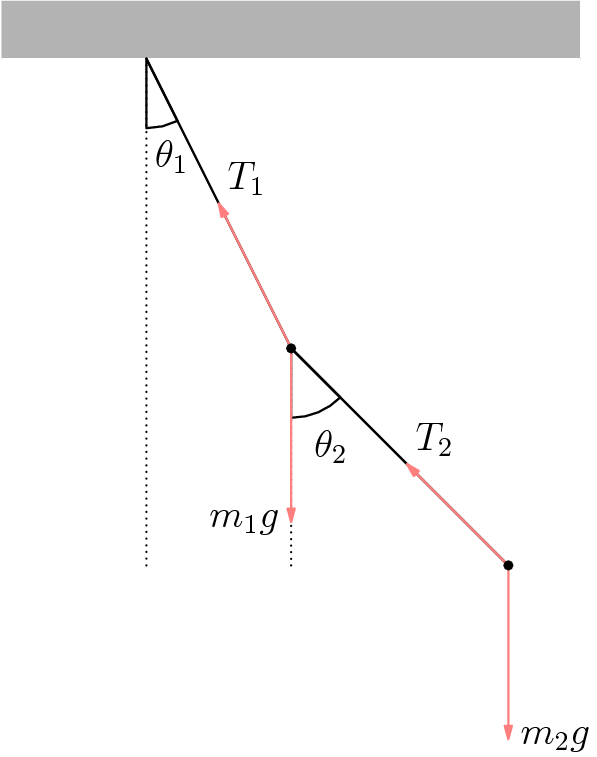
\includegraphics[width=8cm]{P03/double pendulum.png}
\end{center}
Since the angles are small, it holds that 
\[\sin\theta \approx \theta, \quad \cos\theta \approx 1.\]
Let us also define 
\[\sin\theta_1 = \frac{X_1}{L}, \quad \sin\theta_2 = \frac{X_2 - X_1}{L}.\]
The angles are small so $T_1 \approx (M_1 + M_2)g$ (as it holds both masses) and $T_2 \approx M_2 g$ (as it holds only the mass $M_2$). We can now write our equations of motion. We can start with the lower mass. The only force that attempts to bring the second mass back to
equilibrium is the horizontal component of $T_2$. Therefore, we have
\[M_2 \ddot{X}_2  = -T_2\sin\theta_2 = -\frac{M_2g}{\ell} (X_2 - X_1).\]
If we define $\omega^2 \equiv g/L$, we find 
\[\ddot{X}_2 + \omega_0^2 X_2 - \omega_0^2 X_1 = 0.\]
For the first mass, we have two forces. Although not labeled in the diagram there is a component $T_2$ that is directed along the rod and away from the first mass. Therefore, the two forces $T_1$ and $T_2$ fight for equilibrium and our equation of motion can be given as 
\begin{align*}
    M_1\ddot{X}_1 &= -T_1 \sin\theta_1 + T_2 \sin \theta_2 \\ 
     M_1 \ddot{X}_1 &= -2(M_1 + M_2)g \frac{X_1}{L} + M_2g\frac{X_2 - X_1}{L} \\
   0 &= \ddot{X}_1 + \frac{M_1 + 2M_2}{M_1}X_1\omega_0^2 - \frac{M_2}{M_1}X_2 \omega_0^2 
\end{align*}

   \item Using the definition of a normal mode 
\[
\begin{pmatrix}
X_1 \\
X_2 
\end{pmatrix}
= 
\Re \left[
\begin{pmatrix}
A_1 \\
A_2 
\end{pmatrix}
e^{i (\omega t + \phi)}
\right]
\]
we can rearrange to find that 
\begin{align*}
    0 &= \left(\frac{M_1 + 2M_2}{M_1}\omega_0^2 - \omega^2\right)A_1 - \frac{M_2}{M_1}\omega_0^2 A_2\\
    0 &= -\omega_0^2 A_1 + \left(\omega_0^2 - \omega^2\right)
\end{align*}
Now, rewrite in matrix format 
\[
\begin{pmatrix}
 \frac{M_1 + 2M_2}{M_1}\omega_0^2 - \omega^2 & -\frac{M_2}{M_1}\omega_0^2 \\ 
 -\omega_0^2 & \omega_0^2 - \omega^2
\end{pmatrix}
\begin{pmatrix}
A_1 \\
A_2
\end{pmatrix}
=0.
\]
To get a solution, we need to solve the equation where the determinant of the left matrix is zero.
\[
\begin{vmatrix}
\frac{M_1 + 2M_2}{M_1}\omega_0^2 - \omega^2 & -\frac{M_2}{M_1}\omega_0^2 \\ 
 -\omega_0^2 & \omega_0^2 - \omega^2
\end{vmatrix}
= 0.
\]
\[\left(\frac{M_1 + 2M_2}{M_1}\omega_0^2 - \omega^2\right)\left(\omega_0^2 - \omega^2\right) - \frac{M_2}{M_1}\omega_0^4 = 0\]
Rearranging yields the equation 
\[\omega^4 - \frac{2 (M_1 + M_2)}{M_1}\omega_0^2 \omega^2 + \frac{M_1 + M_2}{M_1}\omega_0^4 = 0.\]
Using substitution tells us that the roots of this equation are 
$$ \omega^2 = \frac{(M_2+M_1) \pm \sqrt {M_2^2 + M_1M_2}}{M1} \omega_0^2 \implies \omega^2 = (1+\alpha) \pm \sqrt {1+ \alpha^2}$$
Here we used $\alpha = \frac{M_2}{M_1}$
\end{enumerate}
\end{sol}
\begin{sol}
The main argument of the stationary phase principle is that if the phase changes too quickly, the integral will cancel out over the function. Thus, where the function peaks, $\frac{\partial \phi}{\partial k} = 0$, where $\phi$ is the phase.
\begin{enumerate}[label=\textbf{(\alph*)}]
\item $$\Psi(x) = \int_{-\infty}^{\infty}\mathrm{d}k\;\exp(-L^2(k - k_0)^2 + ikx)  = \int_{-\infty}^{\infty}\mathrm{d}k\;\exp(-L^2k^2 + 2L^2kk_0 - L^2k_0^2 + ikx)$$The phase part of the exponent is the imaginary term, so:
$$\frac{\partial}{\partial k}(ikx) = ix = 0 \implies x = 0$$This can be confirmed by actually evaluating the integral:
\begin{align*}
\Psi(x) &= \int_{-\infty}^{\infty}\mathrm{d}k\;\exp(-L^2k^2 + (2L^2k_0 + ix)k- L^2k_0^2) \\
&= \sqrt{\frac{\pi}{L^2}}\exp(L^2k_0^2)\exp((2L^2k_0 + ix)^2/4L^2) \\
&= \frac{\sqrt{\pi}}{L}\exp(L^2k_0^2)\exp(L^2k_0^2)\exp(ik_0x)\exp(-x^2/4L^2)
\end{align*}
Notice that the last exponential term decays to zero as $x$ moves away from zero, proving our conclusion that the wavefunction peaks at $x = 0$

\item $$\Psi(x) = \int_{-\infty}^{\infty}\mathrm{d}k\;\exp(-L^2(k - k_0)^2-ikx_0+ikx)$$
The wave-function peaks when
$$\frac{\partial}{\partial k}(-ikx_0+ikx) = -ix_0+ix \implies x = x_0$$
Let us try to verify this by evaluating the integral:
\begin{align*}
\Psi(x) &= \int_{-\infty}^{\infty}\mathrm{d}k\;\exp(-L^2k^2 + (2L^2k_0 - ix_0 + ix)k - L^2k_0^2) \\
&= \sqrt{\frac{\pi}{L^2}}\exp(L^2k_0^2)\exp\left(\frac{2L^2k_0 -ix_0+ix)^2}{4L^2}\right) \\
&= \frac{\sqrt{\pi}}{L}\exp(L^2k_0^2)\exp(L^2k_0^2)\exp(ik_0(x-x_0))\exp\left(\frac{-(x-x_0)^2}{4L^2}\right)
% &= \sqrt{\frac{\pi}{L^2}}\exp(4L^4k^2k_0^2/4L^2) \\
% &= \frac{\sqrt{\pi}}{L}\exp(L^2k^2k_0^2)
\end{align*}
Clearly, this wavefunction peaks at $x=x_0$. The extra phase shift introduced simply slides it over by that factor. 
\end{enumerate}
\end{sol}
\begin{sol}
\begin{enumerate}[label=\textbf{(\alph*)}]
\item On displacing by a distance $x$ from the equilibrium position, both springs will have a spring force directed towards the equilibrium position. This means that we have $$F_{\text{net}}= -(2Kx + Kx)\hat{x} = -3Kx\hat{x}.$$ 
Now, we write Newton's second law, and get rid of $\hat{x}$ as all the forces are in the $x$-direction to yield
\[m\ddot{x} = -3Kx\implies \omega = \boxed{\sqrt{\frac{3K}{M}}}.\]
\item At mean position, $v = A\omega $. Therefore 
\[A= \frac{v}{\omega} = \boxed{{v}\sqrt{\frac{M}{3K}}}.\]
\item We know $$x = A \sin (\omega t + \phi).$$ From initial conditions we know that $\omega = \sqrt{\frac{3K}{M}}$, $A={v}\sqrt{\frac{M}{3K}}$, and $\phi = 0$. Therefore 
$$ x = \boxed{v\sqrt {\frac {M}{3K}} \sin \left( \sqrt {\frac{3K}{M}} t \right)}.$$
\item From the lecture, we see that we can write the position of the center of mass as the complex function 
\[z (t) = \Re \left[Ae^{i (\omega t + \phi)}\right].\]
From initial conditions we know that $\omega = \sqrt{\frac{3K}{M}}$, $A=v\sqrt{\frac{M}{3K}}$, and $\phi = 0$ and therefore we have,
\[z(t) = \boxed{\Re \left[v\sqrt{\frac{M}{3K}}e^{i\sqrt{\frac{3K}{M}}t}\right]}.\]
\end{enumerate}
\end{sol}
\begin{sol}
\begin{enumerate}[label=\textbf{(\alph*)}]
\item Notice that 
\[\int_{-\infty}^{\infty}\dd x |\Psi (x)|^2 = \int_{-\infty}^{\infty}\dd x \Psi (x) \Psi^{*}(x) = \int_{-\infty}^{\infty} \dd x \left( \int_{-\infty}^{\infty} \dd p \Phi (p) e^{ixp}\right)\left(\int_{-\infty}^{\infty} \dd p' \Phi^{*} (p') e^{-ixp'}\right).  \]
This can be rewritten with the dirac delta function, as $\int e^{ix (p - p')} = \delta (p - p')$, so 
\[\int_{-\infty}^{\infty}\dd x\int_{-\infty}^{\infty}\dd p \Phi (p) \int_{-\infty}^{\infty}\dd p' \Phi^{*} (p') \delta (p - p') = \int_{-\infty}^{\infty} \dd p |\Phi (p)|^2.\]
\item Using the standard normalization integral and taking into account the spherical symmetry of the situation: $$\int_{0}^{\infty}\left(Ne^{-r/a_0}\right)^24\pi r^2\;\mathrm{d}r = \int_{0}^{\infty}N^2e^{-2r/a_0}\;4\pi r^2\;\mathrm{d}r = \pi N^2a_0^3 = 1$$ Thus, $$N = \sqrt{\frac{1}{\pi a_0^3}}$$
Using Parseval's theorem gives us a normalization condition for momentum wavefunctions similar to the one used in part b): $$\int_{-\infty}^{\infty}\frac{N'^2}{\left(1 + \frac{a_0^2p^2}{\hbar^2}\right)^4}\;4\pi p^2\;\mathrm{d}p = 1$$ Then, $$\int_{-\infty}^{\infty}\frac{4\pi p^2\;\mathrm{d}p}{\left(1 + \frac{a_0^2p^2}{\hbar^2}\right)^4} = \frac{\pi^2\hbar^3}{8a_0^3} \implies N' = \sqrt{\frac{8a_0^3}{\pi^2\hbar^3}}$$
Using the probabalistic interpretation of the momentum wavefunction, the probability that the \textbf{magnitude} of the momentum exceeds $\hbar/a_0$ is: $$\int_{\hbar/a_0}^{\infty}\frac{N'^2}{\left(1 + \frac{a_0^2p^2}{\hbar^2}\right)^4}\;4\pi p^2\;\mathrm{d}p$$
\end{enumerate}
\end{sol}
\begin{sol}
$|\gamma(t)|$ will continue increasing as the two wavepackets evolve, since their wavefunctions will have more overlap as they spread out.
\end{sol}
\begin{sol}
First note that: $$ J(x) = \frac{\hbar}{m}\operatorname{Im}(\Psi^*(x)\frac{\partial \Psi(x)}{\partial x}) = \frac{\hbar}{2im}(\Psi^*(x)\frac{\partial \Psi(x)}{\partial x} - \Psi(x)\frac{\partial \Psi^*(x)}{\partial x})$$
Then,
\begin{enumerate}[label=\textbf{(\alph*)}]
\item $\Psi(x) = Ae^{\gamma x}$:
\begin{align*}J(x) &= \frac{\hbar}{2im}(A^*e^{\gamma x}\frac{\partial }{\partial x}(Ae^{\gamma x}) - Ae^{\gamma x}\frac{\partial}{\partial x}(A^*e^{\gamma x})) \\ &= \frac{\hbar|A|^2}{2im}(e^{\gamma x}\frac{\partial}{\partial x}(e^{\gamma x}) - e^{\gamma x}\frac{\partial}{\partial x}(e^{\gamma x})) \\ &= 0
\end{align*}
Alternatively,
\begin{align*}
    J(x) &= \frac{\hbar}{m}\operatorname{Im}(A^*e^{\gamma x}\frac{\partial}{\partial x}(Ae^{\gamma x})) \\ &= \frac{\hbar}{m}\operatorname{Im}(AA^*\gamma e^{2\gamma x}) \\ &= 0
\end{align*}
\item $\Psi(x) = N(x)e^{iS(x)/\hbar}$:
\begin{align*}
    J(x) &= \frac{\hbar}{2im}(N(x)e^{-iS(x)/\hbar}\frac{\partial}{\partial x}(N(x)e^{iS(x)/\hbar}) - N(x)e^{iS(x)/\hbar}\frac{\partial}{\partial x}(N(x)e^{-iS(x)/\hbar})) \\ &= \frac{1}{m}N(x)^2\frac{\partial S(x)}{\partial x}
\end{align*}
Alternatively,
\begin{align*}
    J(x) &= \frac{\hbar}{m}\operatorname{Im}(N(x)e^{-iS(x)/\hbar}\frac{\partial}{\partial x}(N(x)e^{iS(x)/\hbar})) \\ &= \frac{\hbar}{m}\operatorname{Im}(N(x)^2 * i\frac{\partial S(x)}{\partial x}/\hbar) \\ &= \frac{1}{m}N(x)^2\frac{\partial S(x)}{\partial x}
\end{align*}
\item $\Psi(x) = Ae^{ikx} + Be^{-ikx}$:
\begin{align*}
    J(x) &= \frac{\hbar}{2im}((A^*e^{-ikx} + B^*e^{ikx})\frac{\partial}{\partial x}(Ae^{ikx} + Be^{-ikx}) - (Ae^{ikx} + Be^{-ikx})\frac{\partial}{\partial x}(A^*e^{-ikx} + B^*e^{ikx})) \\ &= \frac{\hbar k}{m}(AA^* - BB^*) \\ &= \frac{\hbar k}{m}(|A|^2 - |B|^2)
\end{align*}
Alternatively,
\begin{align*}
    J(x) &= \frac{\hbar}{m}\operatorname{Im}((A^*e^{-ikx} + B^*e^{ikx})\frac{\partial}{\partial x}(Ae^{ikx} + Be^{-ikx})) \\ &= \frac{\hbar}{m}(AA^* - BB^*) \\ &= \frac{\hbar}{m}(|A|^2 - |B|^2)
\end{align*}

\end{enumerate}
\end{sol}


\newpage
\section*{Problem Set 7}
\begin{sol}
\begin{enumerate}[label=\textbf{(\alph*)}] 
\item We begin by first drawing a diagram:
\begin{center}
    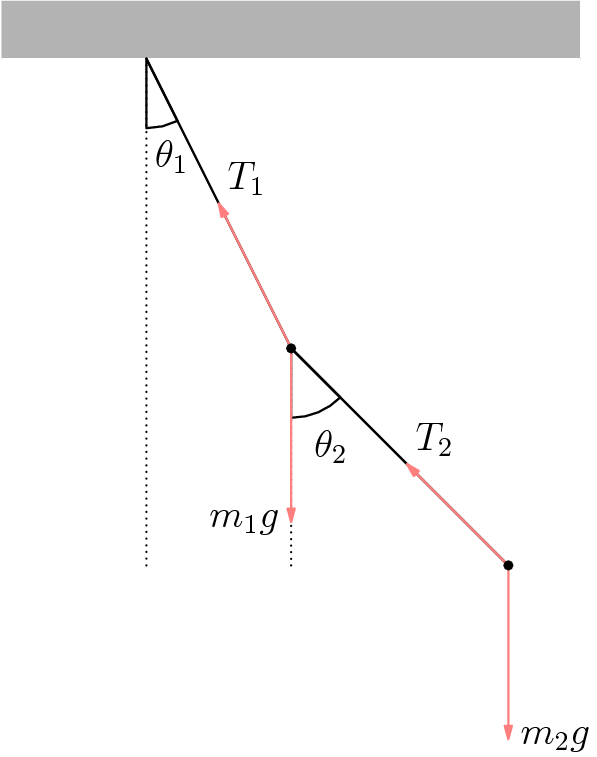
\includegraphics[width=8cm]{P03/double pendulum.png}
\end{center}
Since the angles are small, it holds that 
\[\sin\theta \approx \theta, \quad \cos\theta \approx 1.\]
Let us also define 
\[\sin\theta_1 = \frac{X_1}{L}, \quad \sin\theta_2 = \frac{X_2 - X_1}{L}.\]
The angles are small so $T_1 \approx (M_1 + M_2)g$ (as it holds both masses) and $T_2 \approx M_2 g$ (as it holds only the mass $M_2$). We can now write our equations of motion. We can start with the lower mass. The only force that attempts to bring the second mass back to
equilibrium is the horizontal component of $T_2$. Therefore, we have
\[M_2 \ddot{X}_2  = -T_2\sin\theta_2 = -\frac{M_2g}{\ell} (X_2 - X_1).\]
If we define $\omega^2 \equiv g/L$, we find 
\[\ddot{X}_2 + \omega_0^2 X_2 - \omega_0^2 X_1 = 0.\]
For the first mass, we have two forces. Although not labeled in the diagram there is a component $T_2$ that is directed along the rod and away from the first mass. Therefore, the two forces $T_1$ and $T_2$ fight for equilibrium and our equation of motion can be given as 
\begin{align*}
    M_1\ddot{X}_1 &= -T_1 \sin\theta_1 + T_2 \sin \theta_2 \\ 
     M_1 \ddot{X}_1 &= -2(M_1 + M_2)g \frac{X_1}{L} + M_2g\frac{X_2 - X_1}{L} \\
   0 &= \ddot{X}_1 + \frac{M_1 + 2M_2}{M_1}X_1\omega_0^2 - \frac{M_2}{M_1}X_2 \omega_0^2 
\end{align*}

   \item Using the definition of a normal mode 
\[
\begin{pmatrix}
X_1 \\
X_2 
\end{pmatrix}
= 
\Re \left[
\begin{pmatrix}
A_1 \\
A_2 
\end{pmatrix}
e^{i (\omega t + \phi)}
\right]
\]
we can rearrange to find that 
\begin{align*}
    0 &= \left(\frac{M_1 + 2M_2}{M_1}\omega_0^2 - \omega^2\right)A_1 - \frac{M_2}{M_1}\omega_0^2 A_2\\
    0 &= -\omega_0^2 A_1 + \left(\omega_0^2 - \omega^2\right)
\end{align*}
Now, rewrite in matrix format 
\[
\begin{pmatrix}
 \frac{M_1 + 2M_2}{M_1}\omega_0^2 - \omega^2 & -\frac{M_2}{M_1}\omega_0^2 \\ 
 -\omega_0^2 & \omega_0^2 - \omega^2
\end{pmatrix}
\begin{pmatrix}
A_1 \\
A_2
\end{pmatrix}
=0.
\]
To get a solution, we need to solve the equation where the determinant of the left matrix is zero.
\[
\begin{vmatrix}
\frac{M_1 + 2M_2}{M_1}\omega_0^2 - \omega^2 & -\frac{M_2}{M_1}\omega_0^2 \\ 
 -\omega_0^2 & \omega_0^2 - \omega^2
\end{vmatrix}
= 0.
\]
\[\left(\frac{M_1 + 2M_2}{M_1}\omega_0^2 - \omega^2\right)\left(\omega_0^2 - \omega^2\right) - \frac{M_2}{M_1}\omega_0^4 = 0\]
Rearranging yields the equation 
\[\omega^4 - \frac{2 (M_1 + M_2)}{M_1}\omega_0^2 \omega^2 + \frac{M_1 + M_2}{M_1}\omega_0^4 = 0.\]
Using substitution tells us that the roots of this equation are 
$$ \omega^2 = \frac{(M_2+M_1) \pm \sqrt {M_2^2 + M_1M_2}}{M1} \omega_0^2 \implies \omega^2 = (1+\alpha) \pm \sqrt {1+ \alpha^2}$$
Here we used $\alpha = \frac{M_2}{M_1}$
\end{enumerate}
\end{sol}
\begin{sol}
The main argument of the stationary phase principle is that if the phase changes too quickly, the integral will cancel out over the function. Thus, where the function peaks, $\frac{\partial \phi}{\partial k} = 0$, where $\phi$ is the phase.
\begin{enumerate}[label=\textbf{(\alph*)}]
\item $$\Psi(x) = \int_{-\infty}^{\infty}\mathrm{d}k\;\exp(-L^2(k - k_0)^2 + ikx)  = \int_{-\infty}^{\infty}\mathrm{d}k\;\exp(-L^2k^2 + 2L^2kk_0 - L^2k_0^2 + ikx)$$The phase part of the exponent is the imaginary term, so:
$$\frac{\partial}{\partial k}(ikx) = ix = 0 \implies x = 0$$This can be confirmed by actually evaluating the integral:
\begin{align*}
\Psi(x) &= \int_{-\infty}^{\infty}\mathrm{d}k\;\exp(-L^2k^2 + (2L^2k_0 + ix)k- L^2k_0^2) \\
&= \sqrt{\frac{\pi}{L^2}}\exp(L^2k_0^2)\exp((2L^2k_0 + ix)^2/4L^2) \\
&= \frac{\sqrt{\pi}}{L}\exp(L^2k_0^2)\exp(L^2k_0^2)\exp(ik_0x)\exp(-x^2/4L^2)
\end{align*}
Notice that the last exponential term decays to zero as $x$ moves away from zero, proving our conclusion that the wavefunction peaks at $x = 0$

\item $$\Psi(x) = \int_{-\infty}^{\infty}\mathrm{d}k\;\exp(-L^2(k - k_0)^2-ikx_0+ikx)$$
The wave-function peaks when
$$\frac{\partial}{\partial k}(-ikx_0+ikx) = -ix_0+ix \implies x = x_0$$
Let us try to verify this by evaluating the integral:
\begin{align*}
\Psi(x) &= \int_{-\infty}^{\infty}\mathrm{d}k\;\exp(-L^2k^2 + (2L^2k_0 - ix_0 + ix)k - L^2k_0^2) \\
&= \sqrt{\frac{\pi}{L^2}}\exp(L^2k_0^2)\exp\left(\frac{2L^2k_0 -ix_0+ix)^2}{4L^2}\right) \\
&= \frac{\sqrt{\pi}}{L}\exp(L^2k_0^2)\exp(L^2k_0^2)\exp(ik_0(x-x_0))\exp\left(\frac{-(x-x_0)^2}{4L^2}\right)
% &= \sqrt{\frac{\pi}{L^2}}\exp(4L^4k^2k_0^2/4L^2) \\
% &= \frac{\sqrt{\pi}}{L}\exp(L^2k^2k_0^2)
\end{align*}
Clearly, this wavefunction peaks at $x=x_0$. The extra phase shift introduced simply slides it over by that factor. 
\end{enumerate}
\end{sol}

\section*{Problem Set 8}
\begin{sol}
\begin{enumerate}[label=\textbf{(\alph*)}]
\item Notice that 
\[\int_{-\infty}^{\infty}\dd x |\Psi (x)|^2 = \int_{-\infty}^{\infty}\dd x \Psi (x) \Psi^{*}(x) = \int_{-\infty}^{\infty} \dd x \left( \int_{-\infty}^{\infty} \dd p \Phi (p) e^{ixp}\right)\left(\int_{-\infty}^{\infty} \dd p' \Phi^{*} (p') e^{-ixp'}\right).  \]
This can be rewritten with the dirac delta function, as $\int e^{ix (p - p')} = \delta (p - p')$, so 
\[\int_{-\infty}^{\infty}\dd x\int_{-\infty}^{\infty}\dd p \Phi (p) \int_{-\infty}^{\infty}\dd p' \Phi^{*} (p') \delta (p - p') = \int_{-\infty}^{\infty} \dd p |\Phi (p)|^2.\]
\item Using the standard normalization integral and taking into account the spherical symmetry of the situation: $$\int_{0}^{\infty}\left(Ne^{-r/a_0}\right)^24\pi r^2\;\mathrm{d}r = \int_{0}^{\infty}N^2e^{-2r/a_0}\;4\pi r^2\;\mathrm{d}r = \pi N^2a_0^3 = 1$$ Thus, $$N = \sqrt{\frac{1}{\pi a_0^3}}$$
Using Parseval's theorem gives us a normalization condition for momentum wavefunctions similar to the one used in part b): $$\int_{-\infty}^{\infty}\frac{N'^2}{\left(1 + \frac{a_0^2p^2}{\hbar^2}\right)^4}\;4\pi p^2\;\mathrm{d}p = 1$$ Then, $$\int_{-\infty}^{\infty}\frac{4\pi p^2\;\mathrm{d}p}{\left(1 + \frac{a_0^2p^2}{\hbar^2}\right)^4} = \frac{\pi^2\hbar^3}{8a_0^3} \implies N' = \sqrt{\frac{8a_0^3}{\pi^2\hbar^3}}$$
Using the probabalistic interpretation of the momentum wavefunction, the probability that the \textbf{magnitude} of the momentum exceeds $\hbar/a_0$ is: $$\int_{\hbar/a_0}^{\infty}\frac{N'^2}{\left(1 + \frac{a_0^2p^2}{\hbar^2}\right)^4}\;4\pi p^2\;\mathrm{d}p$$
\end{enumerate}
\end{sol}
\end{document}
